\documentclass[10pt,a4paper]{article}
\usepackage[margin=1.45cm]{geometry}
\usepackage[T1]{fontenc}
\usepackage[utf8]{inputenc}
\usepackage{lmodern}
\usepackage{amsmath,amssymb,bm}
\usepackage{enumitem}
\usepackage{tabularx,array,booktabs,multicol}
\usepackage[most]{tcolorbox}
\usepackage{titlesec}
\usepackage{fancyhdr}
\usepackage[hidelinks]{hyperref}
\usepackage{xcolor}
\usepackage{tikz}
\usetikzlibrary{arrows.meta,positioning}
\setlength{\parindent}{0pt}
\setlength{\parskip}{3pt}
\setlist[itemize]{nosep,leftmargin=5mm}
\setlist[enumerate]{nosep,leftmargin=6mm}
\pagestyle{fancy}\fancyhf{}\lhead{EM1 - opgavebaseret formelsamling}\rhead{Master}\cfoot{\thepage}
\titleformat{\section}{\large\bfseries}{\thesection}{0.6em}{}
\titleformat{\subsection}{\normalsize\bfseries}{\thesubsection}{0.55em}{}
\newtcolorbox{taskbox}[1]{breakable,colback=white,colframe=black!65,boxrule=0.5pt,arc=1mm,title=\textbf{#1},fonttitle=\normalsize,left=2mm,right=2mm,top=1.2mm,bottom=1.2mm}
\newtcolorbox{quickbox}[1]{colback=black!3,colframe=black!45,boxrule=0.4pt,arc=1mm,title=\textbf{#1},left=2mm,right=2mm,top=1mm,bottom=1mm}
\newtcolorbox{casebox}[1]{breakable,colback=white,colframe=black!52,boxrule=0.45pt,arc=1mm,title=\textbf{#1},fonttitle=\small,left=1.8mm,right=1.8mm,top=1.0mm,bottom=1.0mm}
\newcommand{\casemethod}[1]{\par\smallskip{\footnotesize\textbf{Fremgangsmåde:} #1}}
\newcommand{\casepitfall}[1]{\par\smallskip{\footnotesize\textbf{Faldgrube:} #1}}
\newcommand{\epsz}{\varepsilon_0}
\newcommand{\examlabel}[1]{\par\medskip\noindent{\footnotesize\bfseries\textsf{#1}}\par\vspace{0.4mm}}
\definecolor{Efield}{RGB}{198,112,24}
\definecolor{PosCharge}{RGB}{180,55,45}
\definecolor{NegCharge}{RGB}{55,105,170}
\definecolor{GaussGray}{RGB}{120,120,120}
\definecolor{ConductorGray}{RGB}{225,225,225}
\definecolor{DielectricTint}{RGB}{225,239,242}
\newcommand{\chaptertag}[1]{\hfill{\footnotesize\color{black!50}\textit{#1}}}
\newcommand{\atlasrule}{\par\vspace{1mm}\hrule\vspace{2mm}}
\begin{document}

\begin{center}
{\LARGE\bfseries Elektromagnetisme 1}\\[1mm]
{\large Opgavebaseret formelsamling - master}\\[2mm]
\small Bygget på den eksisterende EM1-formelsamling, men organiseret efter eksamensopgavetyper.\\
\end{center}
\vspace{-2mm}
\hrule
\vspace{2mm}

\begin{quickbox}{Sådan bruges arket - den fysiske struktur}
Find først \textbf{DEL + opgavetype}. Brug samme flow: \textbf{kilde} $\to$ \textbf{potentiale} $\to$ \textbf{felt} $\to$ \textbf{kraft}, når det er relevant.
\[
\boxed{\text{DEL I: elektrostatik}}\ \longrightarrow\
\boxed{\text{DEL II: magnetostatik}}\ \longrightarrow\
\boxed{\text{DEL III: elektrodynamik}}
\]
\[
\boxed{\rho\to V\to\mathbf E\to\mathbf F}
\qquad\qquad
\boxed{\mathbf J\to\mathbf A\to\mathbf B\to\mathbf F}.
\]
Under eksamen: \textbf{se figur} $\to$ \textbf{genkend} $\to$ \textbf{metode} $\to$ \textbf{regning} $\to$ \textbf{kontrol}.
\end{quickbox}

\tableofcontents
\newpage

\section{Hurtigt matematisk værktøj}
\begin{multicols}{2}
\textbf{Krydsprodukt}
\[
\hat x\times\hat y=\hat z,\quad \hat y\times\hat z=\hat x,\quad \hat z\times\hat x=\hat y,
\]
omvendt rækkefølge giver minus; samme vektor krydset med sig selv giver 0.

\textbf{Ladningselementer}
\[
dq=\lambda\,dl,\qquad dq=\sigma\,da,\qquad dq=\rho\,d\tau.
\]

\textbf{Volumenelementer}
\[
d\tau=dx\,dy\,dz,
\]
\[
d\tau=s\,ds\,d\phi\,dz,
\]
\[
d\tau=r^2\sin\theta\,dr\,d\theta\,d\phi.
\]

\textbf{Grundrelationer}
\[
\nabla\cdot\mathbf E=\frac{\rho}{\epsz},\qquad \nabla\times\mathbf E=0,
\]
\[
\nabla\cdot\mathbf B=0,\qquad \nabla\times\mathbf B=\mu_0\mathbf J\quad\text{(magnetostatik)}.
\]
\end{multicols}

\section*{DEL I - ELEKTRISKE FELTER / POTENTIALE}
\phantomsection
\addcontentsline{toc}{section}{DEL I - ELEKTRISKE FELTER / POTENTIALE}
\begin{center}
{\Large\bfseries E/V - visuelt problemløsningsatlas}\\[1mm]
{\small Først værktøjerne $\to$ derefter geometri/opgavetype. $E$ og $V$ vises sammen, når de hører til samme fysiske case.}
\end{center}
\vspace{1mm}
\begin{quickbox}{Sådan navigerer du E/V-delen}
\[
\boxed{\text{hvad er givet?}}
\to
\boxed{\text{genkend geometrien}}
\to
\boxed{\text{vælg metode}}
\to
\boxed{E\text{ eller }V}
\to
\boxed{\text{regn videre}}
\]
\begin{center}
\begin{tabular}{llll}
\textbf{EV0 Værktøjer} & \textbf{EV1 Felt-tests} & \textbf{EV2 Find $E/V$} & \textbf{EV3 Regioner}\\
\textbf{EV4 Ledere/hulrum} & \textbf{EV5 Randværdier} & \textbf{EV6 Multipoler} & \textbf{EV7 Materialer}
\end{tabular}
\end{center}
\end{quickbox}

\newpage
\section*{EV0 - Grundligninger og centrale relationer}
\phantomsection
\addcontentsline{toc}{section}{EV0 - Grundligninger og centrale relationer}
\begin{multicols}{2}
\begin{quickbox}{Kilder $\to$ felt}
\[
\boxed{\mathbf E(\mathbf r)=\frac{1}{4\pi\varepsilon_0}\frac{q}{R^2}\hat{\mathbf R}}
\]
\[
\mathbf E_{\rm tot}=\sum_i\mathbf E_i,
\qquad
 dq=\lambda dl,\\;dq=\sigma da,\\;dq=\rho d\tau.
\]
\[
\boxed{\mathbf E=\frac{1}{4\pi\varepsilon_0}\int\frac{\mathbf R}{R^3}\\,dq}
\]
\end{quickbox}
\begin{quickbox}{Gauss og kilde-test}
\[
\boxed{\oint\mathbf E\cdot d\mathbf a=\frac{Q_{\rm enc}}{\varepsilon_0}},
\qquad
\boxed{\nabla\cdot\mathbf E=\frac{\rho}{\varepsilon_0}}
\]
\[
\boxed{\rho=\varepsilon_0\nabla\cdot\mathbf E}.
\]
\end{quickbox}
\begin{quickbox}{Potentiale}
\[
\boxed{V=\frac{1}{4\pi\varepsilon_0}\int\frac{dq}{R}}
\]
\[
\boxed{V(B)-V(A)=-\int_A^B\mathbf E\cdot d\mathbf l},
\qquad
\boxed{\mathbf E=-\nabla V}.
\]
\end{quickbox}
\begin{quickbox}{Poisson / Laplace}
\[
\boxed{\nabla^2V=-\frac{\rho}{\varepsilon_0}},
\qquad
\boxed{\rho=0\Rightarrow\nabla^2V=0}.
\]
\end{quickbox}
\begin{quickbox}{Arbejde og energi}
\[
U=qV,
\qquad W_{\rm felt}=-\Delta U,
\qquad W_{\rm ekst}=\Delta U.
\]
\[
U=\frac{1}{4\pi\varepsilon_0}\sum_{i<j}\frac{q_iq_j}{r_{ij}}.
\]
I vakuum:
\[
\boxed{U_E=\frac{\varepsilon_0}{2}\iiint E^2\\,d\tau}.
\]
\end{quickbox}
\begin{quickbox}{Kapacitans}
\[
\boxed{C=\frac{Q}{\Delta V}},
\qquad
\boxed{U_C=\frac12C(\Delta V)^2=\frac{Q^2}{2C}=\frac12Q\Delta V}.
\]
\end{quickbox}
\end{multicols}

\newpage
\section*{EV1 - Maxwell-ligninger og felt-tests}
\phantomsection
\addcontentsline{toc}{section}{EV1 - Maxwell-ligninger og felt-tests}
\begin{casebox}{De fire fulde Maxwell-ligninger - differentialform}
\[
\boxed{\nabla\cdot\mathbf E=\frac{\rho}{\varepsilon_0}},
\qquad
\boxed{\nabla\cdot\mathbf B=0},
\]
\[
\boxed{\nabla\times\mathbf E=-\frac{\partial\mathbf B}{\partial t}},
\qquad
\boxed{\nabla\times\mathbf B=\mu_0\mathbf J+\mu_0\varepsilon_0\frac{\partial\mathbf E}{\partial t}}.
\]
\end{casebox}
\begin{casebox}{Samme ligninger - integralform}
\[
\boxed{\oint_S\mathbf E\cdot d\mathbf a=\frac{Q_{\rm enc}}{\varepsilon_0}},
\qquad
\boxed{\oint_S\mathbf B\cdot d\mathbf a=0},
\]
\[
\boxed{\oint_C\mathbf E\cdot d\mathbf l=-\frac{d}{dt}\iint_S\mathbf B\cdot d\mathbf a},
\]
\[
\boxed{\oint_C\mathbf B\cdot d\mathbf l=\mu_0I_{\rm enc}+\mu_0\varepsilon_0\frac{d}{dt}\iint_S\mathbf E\cdot d\mathbf a}.
\]
\end{casebox}
\begin{quickbox}{Recognition / felt-test}
\[
\nabla\cdot\mathbf E\to\rho,
\qquad
\nabla\times\mathbf E=0\to\text{muligt elektrostatisk felt},
\]
\[
\nabla\times\mathbf E\neq0\to\text{tidsvarierende }\mathbf B.
\]
I en ren elektrostatisk opgave skal $\partial\mathbf B/\partial t=0$, så $\nabla\times\mathbf E=0$.
\end{quickbox}

\newpage
\section*{EV2 - Find $E$ eller $V$ ud fra geometri}
\phantomsection
\addcontentsline{toc}{section}{EV2 - Find E/V fra geometri}
\begin{quickbox}{Beslutningstræ}
\[
\begin{array}{rcl}
\text{få punktladninger} &\to& \text{Coulomb + superposition}\\
\text{kontinuert fordeling, lav symmetri} &\to& \text{Coulomb-/potentialintegral}\\
\text{kugle/cylinder/plan, høj symmetri} &\to& \text{Gauss}\\
V\text{ givet} &\to& -\nabla V\\
\mathbf E\text{ givet} &\to& -\int\mathbf E\cdot d\mathbf l
\end{array}
\]
\end{quickbox}
\section*{EV0 - Potentiale: tre veje mellem kilde, $V$ og $E$ \chaptertag{Kap. 2}}
\phantomsection
\addcontentsline{toc}{section}{EV0 - Potentiale: kilde / E / V}

\begin{casebox}{Punktladning og flere punktladninger}
\begin{center}
\begin{minipage}[t]{0.48\linewidth}\centering
\textbf{Én punktladning}\\[1mm]
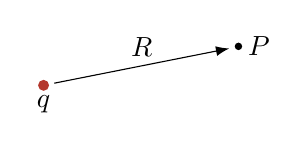
\begin{tikzpicture}[scale=0.9,>=Latex]
  \fill[PosCharge] (-1.4,0) circle (2.2pt) node[below,text=black] {$q$}; \fill (1.35,0.55) circle (1.5pt) node[right] {$P$};
  \draw[->] (-1.25,0.03)--(1.22,0.52) node[midway,above] {$R$};
\end{tikzpicture}
\[
 \boxed{V=k\frac{q}{R}}.
\]
\end{minipage}\hfill
\begin{minipage}[t]{0.48\linewidth}\centering
\textbf{Flere punktladninger}\\[1mm]
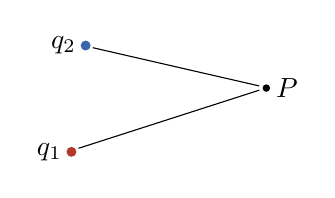
\begin{tikzpicture}[scale=0.9]
  \fill[PosCharge] (-1.4,-0.65) circle (2pt) node[left,text=black] {$q_1$}; \fill[NegCharge] (-1.2,0.85) circle (2pt) node[left,text=black] {$q_2$}; \fill (1.35,0.25) circle (1.5pt) node[right] {$P$};
  \draw (-1.3,-0.60)--(1.25,0.22); \draw (-1.1,0.82)--(1.25,0.28);
\end{tikzpicture}
\[
 \boxed{V=k\sum_i\frac{q_i}{R_i}}.
\]
\[
 \boxed{\text{Potentiale summeres som skalar}}.
\]
\end{minipage}
\end{center}
\end{casebox}

\begin{casebox}{Kontinuert fordeling: samme $dq$-valg som ved Coulomb}
\begin{minipage}[c]{0.48\linewidth}\centering
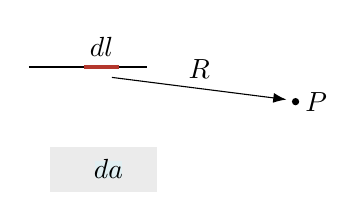
\begin{tikzpicture}[scale=0.88,>=Latex]
  \draw[thick] (-2.1,0.8)--(-0.4,0.8); \draw[very thick,PosCharge] (-1.3,0.8)--(-0.8,0.8) node[midway,above,text=black] {$dl$};
  \fill[black!8] (-1.8,-1.0) rectangle (-0.25,-0.35); \fill[DielectricTint] (-1.15,-0.80) rectangle (-0.75,-0.55); \node at (-0.95,-0.67) {$da$};
  \fill (1.75,0.3) circle (1.5pt) node[right] {$P$}; \draw[->] (-0.9,0.65)--(1.62,0.33) node[midway,above] {$R$};
\end{tikzpicture}
\end{minipage}\hfill
\begin{minipage}[c]{0.48\linewidth}
\[
 \boxed{V(\mathbf r)=k\int\frac{dq}{R}}.
\]
\[
 dq=\lambda\,dl,\qquad dq=\sigma\,da,\qquad dq=\rho\,d\tau.
\]
\casemethod{potentialet er skalar; integrér direkte, og brug geometrien til at skrive $R$.}
\end{minipage}
\end{casebox}

\begin{casebox}{Kendt felt $\leftrightarrow$ kendt potentiale}
\begin{center}
\begin{minipage}[t]{0.48\linewidth}\centering
\textbf{Kendt $\mathbf E$}\\[1mm]
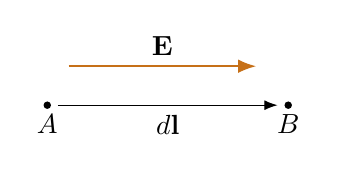
\begin{tikzpicture}[scale=0.9,>=Latex]
  \fill (-1.7,0) circle (1.5pt) node[below] {$A$}; \fill (1.7,0) circle (1.5pt) node[below] {$B$};
  \draw[->,Efield,thick] (-1.4,0.55)--(1.25,0.55) node[midway,above,text=black] {$\mathbf E$}; \draw[->] (-1.55,0)--(1.55,0) node[midway,below] {$d\mathbf l$};
\end{tikzpicture}
\[
 \boxed{V(B)-V(A)=-\int_A^B\mathbf E\cdot d\mathbf l}.
\]
\end{minipage}\hfill
\begin{minipage}[t]{0.48\linewidth}\centering
\textbf{Kendt $V$}\\[1mm]
\[
 \boxed{\mathbf E=-\nabla V}.
\]
Ved radialt potentiale:
\[
 \boxed{V=V(r)\Rightarrow \mathbf E=-\frac{dV}{dr}\hat r}.
\]
\[
 \mathbf E\text{ peger fra højt }V\text{ mod lavt }V.
\]
\end{minipage}
\end{center}
\casepitfall{i elektrostatik er $\nabla\times\mathbf E=0$, så potentialforskellen afhænger kun af endepunkterne.}
\end{casebox}

% ============================================================
\newpage
\section*{EV0 - Energi, arbejde og kapacitans \chaptertag{Kap. 2 + 4}}
\phantomsection
\addcontentsline{toc}{section}{EV0 - Energi, arbejde og kapacitans}

\begin{casebox}{Ladning i eksternt potentiale}
\begin{minipage}[c]{0.42\linewidth}\centering
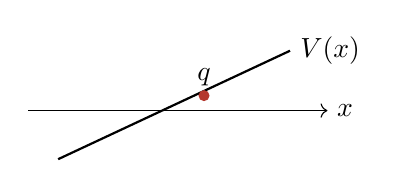
\begin{tikzpicture}[scale=0.95]
  \draw[->] (-2,0)--(2,0) node[right] {$x$}; \draw[thick] (-1.6,-0.65)--(1.5,0.8) node[right] {$V(x)$};
  \fill[PosCharge] (0.35,0.2) circle (2.1pt) node[above,text=black] {$q$};
\end{tikzpicture}
\end{minipage}\hfill
\begin{minipage}[c]{0.54\linewidth}
\[
 \boxed{U=qV_{\rm ekst}}.
\]
\[
 W_{\rm felt}=-\Delta U,\qquad W_{\rm ekst}=\Delta U
\]
for quasistatisk flytning / samme start- og sluthastighed.
\end{minipage}
\end{casebox}

\begin{casebox}{System af punktladninger: hvert par én gang}
\begin{minipage}[c]{0.42\linewidth}\centering
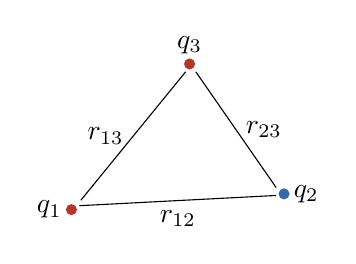
\begin{tikzpicture}[scale=1.0]
  \fill[PosCharge] (-1.3,-0.7) circle (2.0pt) node[left,text=black] {$q_1$};
  \fill[NegCharge] (1.4,-0.5) circle (2.0pt) node[right,text=black] {$q_2$};
  \fill[PosCharge] (0.2,1.15) circle (2.0pt) node[above,text=black] {$q_3$};
  \draw (-1.2,-0.65)--(1.3,-0.52) node[midway,below] {$r_{12}$}; \draw (-1.18,-0.58)--(0.15,1.05) node[midway,left] {$r_{13}$}; \draw (1.3,-0.42)--(0.28,1.05) node[midway,right] {$r_{23}$};
\end{tikzpicture}
\end{minipage}\hfill
\begin{minipage}[c]{0.54\linewidth}
\[
 \boxed{U=k\sum_{i<j}\frac{q_iq_j}{r_{ij}}}
 =\frac12\sum_iq_iV_{\rm andre}(\mathbf r_i).
\]
For kontinuert fordeling:
\[
 \boxed{U=\frac12\iiint\rho V\,d\tau}.
\]
\casepitfall{$i<j$ betyder, at hvert par tælles én gang.}
\end{minipage}
\end{casebox}

\begin{casebox}{Kapacitans og kondensatorenergi}
\[
\boxed{C=\frac{Q}{\Delta V}},
\qquad
\boxed{U_C=\frac12C(\Delta V)^2=\frac{Q^2}{2C}=\frac12Q\Delta V}.
\]
I vakuum kan feltenergien skrives
\[
\boxed{U_E=\frac{\varepsilon_0}{2}\iiint E^2\\,d\tau}.
\]
\casemethod{find først $E$ fra geometrien, integrér til $\Delta V$, og brug derefter $C=Q/\Delta V$.}
\end{casebox}

\begin{casebox}{Arbejde mellem to punktladningsafstande}
\[
 \boxed{W_{\rm ekst}=kq_1q_2\left(\frac1{r_f}-\frac1{r_i}\right)},
 \qquad
 \boxed{W_{\rm felt}=-W_{\rm ekst}}.
\]
\end{casebox}

% ============================================================
\newpage
\section*{EV2 - Punktladninger: $E$ og $V$ sammen \chaptertag{Kap. 2}}
\phantomsection
\addcontentsline{toc}{section}{EV2 - Find E/V: punktladninger}

\begin{casebox}{Punktladning: én kilde, ét feltpunkt}
\begin{minipage}[c]{0.43\linewidth}\centering
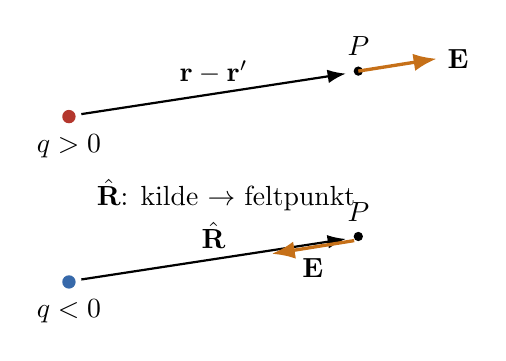
\begin{tikzpicture}[scale=1.05,>=Latex]
  \fill[PosCharge] (-1.9,0) circle (2.3pt) node[below=3pt,text=black] {$q>0$};
  \fill (1.6,0.55) circle (1.6pt) node[above=2pt] {$P$};
  \draw[->,thick] (-1.75,0.03)--(1.45,0.52) node[midway,above] {$\mathbf r-\mathbf r'$};
  \draw[->,Efield,very thick] (1.6,0.55)--(2.55,0.70) node[right,text=black] {$\mathbf E$};
  \node at (0,-0.95) {$\hat{\mathbf R}$: kilde $\to$ feltpunkt};
  \begin{scope}[yshift=-2.0cm]
    \fill[NegCharge] (-1.9,0) circle (2.3pt) node[below=3pt,text=black] {$q<0$};
    \fill (1.6,0.55) circle (1.6pt) node[above=2pt] {$P$};
    \draw[->,thick] (-1.75,0.03)--(1.45,0.52) node[midway,above] {$\hat{\mathbf R}$};
    \draw[->,Efield,very thick] (1.55,0.50)--(0.55,0.34) node[midway,below,text=black] {$\mathbf E$};
  \end{scope}
\end{tikzpicture}
\end{minipage}\hfill
\begin{minipage}[c]{0.53\linewidth}
\[
 k=\frac{1}{4\pi\varepsilon_0},\qquad
 \mathbf R=\mathbf r-\mathbf r',\qquad R=|\mathbf R|.
\]
\[
 \boxed{\mathbf E=k\frac{q}{R^2}\hat{\mathbf R}}
 =k\frac{q}{R^3}\mathbf R.
\qquad\boxed{V=k\frac{q}{R}}
\]
\casemethod{tegn først $\mathbf R$ fra ladningen til observationspunktet. Fortegnet på $q$ bestemmer, om $\mathbf E$ følger eller vender modsat $\hat{\mathbf R}$.}
\casepitfall{$R$ er separationsafstanden mellem kilde og feltpunkt - ikke nødvendigvis koordinaten $r$.}
\end{minipage}
\end{casebox}

\begin{casebox}{Flere punktladninger: vektorsuperposition}
\begin{minipage}[c]{0.48\linewidth}\centering
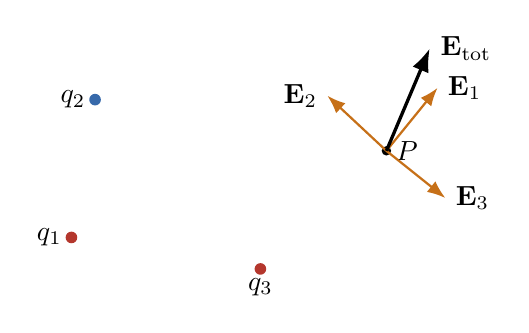
\begin{tikzpicture}[scale=1.0,>=Latex]
  \fill[PosCharge] (-2.0,-0.75) circle (2.1pt) node[left,text=black] {$q_1$};
  \fill[NegCharge] (-1.7,1.0) circle (2.1pt) node[left,text=black] {$q_2$};
  \fill[PosCharge] (0.4,-1.15) circle (2.1pt) node[below,text=black] {$q_3$};
  \fill (2.0,0.35) circle (1.7pt) node[right] {$P$};
  \draw[->,Efield,thick] (2.0,0.35)--(2.65,1.15) node[right,text=black] {$\mathbf E_1$};
  \draw[->,Efield,thick] (2.0,0.35)--(1.25,1.05) node[left,text=black] {$\mathbf E_2$};
  \draw[->,Efield,thick] (2.0,0.35)--(2.75,-0.25) node[right,text=black] {$\mathbf E_3$};
  \draw[->,black,very thick] (2.0,0.35)--(2.55,1.65) node[right] {$\mathbf E_{\rm tot}$};
\end{tikzpicture}
\end{minipage}\hfill
\begin{minipage}[c]{0.48\linewidth}
\[
 \boxed{\mathbf E_{\rm tot}=\sum_i\mathbf E_i}
\qquad\boxed{V_{\rm tot}=k\sum_i\frac{q_i}{R_i}}
\]
\[
 E_x=\sum_iE_{i,x},\qquad E_y=\sum_iE_{i,y},\qquad E_z=\sum_iE_{i,z}.
\]
\[
 \mathbf F=Q\mathbf E_{\rm tot}.
\]
\casemethod{beregn hvert feltbidrag med sin egen retning; brug symmetri før komponentregning.}
\casepitfall{felter summeres som vektorer; potentialer summeres senere som skalarer.}
\end{minipage}
\end{casebox}

\textbf{Gamle opgaver:} nov21.1, feb22.1, feb23.1, nov23.1, feb24.1, jan26.1, N25.2, F22.5.

% ============================================================
\newpage
\section*{EV2 - Kontinuerte ladningsfordelinger \chaptertag{Kap. 2}}
\phantomsection
\addcontentsline{toc}{section}{EV2 - Find E/V: kontinuerte fordelinger}

\begin{casebox}{Linjeladning: $dq=\lambda\,dl'$}
\begin{minipage}[c]{0.47\linewidth}\centering
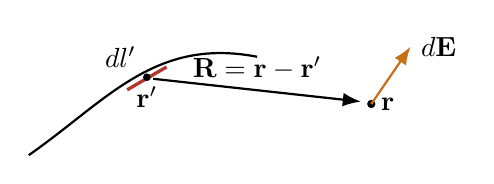
\begin{tikzpicture}[scale=1.0,>=Latex]
  \draw[thick] (-2.2,-0.5) .. controls (-1.2,0.2) and (-0.6,1.0) .. (0.7,0.75);
  \draw[very thick,PosCharge] (-0.95,0.33)--(-0.45,0.62) node[midway,above left,text=black] {$dl'$};
  \fill (-0.70,0.49) circle (1.4pt) node[below] {$\mathbf r'$};
  \fill (2.15,0.15) circle (1.5pt) node[right] {$\mathbf r$};
  \draw[->,thick] (-0.62,0.47)--(2.02,0.18) node[midway,above] {$\mathbf R=\mathbf r-\mathbf r'$};
  \draw[->,Efield,thick] (2.15,0.15)--(2.65,0.88) node[right,text=black] {$d\mathbf E$};
\end{tikzpicture}
\end{minipage}\hfill
\begin{minipage}[c]{0.49\linewidth}
\[
 dq=\lambda\,dl',
\qquad
 d\mathbf E=k\frac{dq}{R^2}\hat{\mathbf R}.
\]
\[
 \boxed{\mathbf E=k\int\frac{\mathbf R}{R^3}\lambda\,dl'}\qquad\boxed{V=k\int\frac{\lambda\,dl'}{R}}.
\]
\casemethod{parametrisér linjen, skriv $\mathbf r'$, derfra $\mathbf R$, og integrér den overlevende feltkomponent.}
\end{minipage}
\end{casebox}

\begin{casebox}{Fladeladning: $dq=\sigma\,da'$}
\begin{minipage}[c]{0.47\linewidth}\centering
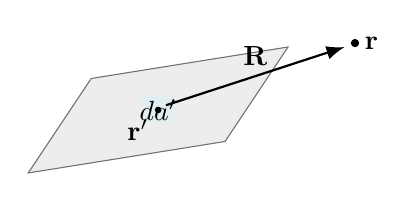
\begin{tikzpicture}[scale=1.0,>=Latex]
  \fill[black!7] (-2.0,-0.8)--(0.5,-0.4)--(1.3,0.8)--(-1.2,0.4)--cycle;
  \draw[black!55] (-2.0,-0.8)--(0.5,-0.4)--(1.3,0.8)--(-1.2,0.4)--cycle;
  \fill[DielectricTint] (-0.55,-0.15) rectangle (-0.15,0.18);
  \node at (-0.35,0.0) {$da'$};
  \fill (-0.35,0.0) circle (1.2pt) node[below left] {$\mathbf r'$};
  \fill (2.15,0.85) circle (1.5pt) node[right] {$\mathbf r$};
  \draw[->,thick] (-0.25,0.06)--(2.02,0.80) node[midway,above] {$\mathbf R$};
\end{tikzpicture}
\end{minipage}\hfill
\begin{minipage}[c]{0.49\linewidth}
\[
 dq=\sigma\,da',
\qquad
 \boxed{\mathbf E=k\iint\frac{\mathbf R}{R^3}\sigma\,da'}\qquad\boxed{V=k\iint\frac{\sigma\,da'}{R}}.
\]
\casemethod{vælg passende fladekoordinater. Ved rotationssymmetri kan fladen ofte opdeles i ringe.}
\end{minipage}
\end{casebox}

\begin{casebox}{Volumenladning: $dq=\rho\,d\tau'$}
\begin{minipage}[c]{0.47\linewidth}\centering
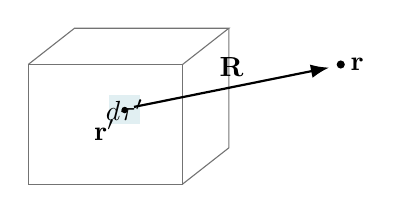
\begin{tikzpicture}[scale=0.98,>=Latex]
  \draw[black!55] (-1.7,-0.9) rectangle (0.3,0.65);
  \draw[black!55] (-1.7,0.65)--(-1.1,1.12)--(0.9,1.12)--(0.3,0.65);
  \draw[black!55] (0.3,-0.9)--(0.9,-0.43)--(0.9,1.12);
  \fill[DielectricTint] (-0.65,-0.12) rectangle (-0.25,0.25);
  \node at (-0.45,0.06) {$d\tau'$};
  \fill (-0.45,0.06) circle (1.2pt) node[below left] {$\mathbf r'$};
  \fill (2.35,0.65) circle (1.5pt) node[right] {$\mathbf r$};
  \draw[->,thick] (-0.33,0.10)--(2.20,0.61) node[midway,above] {$\mathbf R$};
\end{tikzpicture}
\end{minipage}\hfill
\begin{minipage}[c]{0.49\linewidth}
\[
 dq=\rho\,d\tau',
\qquad
 \boxed{\mathbf E=k\iiint\frac{\mathbf R}{R^3}\rho\,d\tau'}\qquad\boxed{V=k\iiint\frac{\rho\,d\tau'}{R}}.
\]
\[
 d\tau'=dx'dy'dz'=s'\,ds'\,d\phi'\,dz'=r'^2\sin\theta'\,dr'\,d\theta'\,d\phi'.
\]
\casemethod{vælg koordinater efter geometrien; brug Gauss i stedet, hvis symmetrien er høj.}
\end{minipage}
\end{casebox}

\begin{quickbox}{Samme geometri i alle kontinuerte Coulomb-integraler}
\[
 \boxed{\mathbf r=\text{feltpunkt}},\qquad
 \boxed{\mathbf r'=\text{kildepunkt}},\qquad
 \boxed{\mathbf R=\mathbf r-\mathbf r'}.
\]
\end{quickbox}

\begin{casebox}{Omvendt case: felt givet, find kilden}
\[
 \boxed{\rho=\varepsilon_0\nabla\cdot\mathbf E}
 \quad\longrightarrow\quad
 \boxed{Q=\iiint\rho\,d\tau}.
\]
\[
 \nabla\times\mathbf E=0\qquad\text{(elektrostatik)}.
\]
\casemethod{tag divergensen af det givne felt; integrér kun hvis der spørges efter total ladning.}
\end{casebox}

% ============================================================
\newpage
\section*{EV2 - Ring og skive på symmetriaksen \chaptertag{Kap. 2}}
\phantomsection
\addcontentsline{toc}{section}{EV2 - Find E/V: ring og skive}
\begin{casebox}{Uniformt ladet ring, radius $R$ - observationspunkt på aksen}
\begin{minipage}[c]{0.43\linewidth}\centering
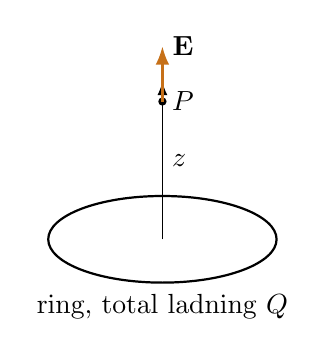
\begin{tikzpicture}[scale=1.0,>=Latex]
  \draw[thick] (0,0) ellipse (1.45 and 0.55); \node at (0,-0.85) {ring, total ladning $Q$};
  \draw[->] (0,0)--(0,2.0) node[midway,right] {$z$}; \fill (0,1.75) circle (1.5pt) node[right] {$P$};
  \draw[->,Efield,thick] (0,1.75)--(0,2.45) node[right,text=black] {$\mathbf E$};
\end{tikzpicture}
\end{minipage}\hfill
\begin{minipage}[c]{0.53\linewidth}
\[
\boxed{V(z)=\frac{1}{4\pi\varepsilon_0}\frac{Q}{\sqrt{z^2+R^2}}}
\]
\[
\boxed{\mathbf E(z)=\frac{1}{4\pi\varepsilon_0}\frac{Qz}{(z^2+R^2)^{3/2}}\hat z}.
\]
\casemethod{alle tværgående feltkomponenter annullerer parvist; kun aksekomponenten overlever.}
\end{minipage}
\end{casebox}
\begin{casebox}{Uniformt ladet skive, radius $R$ - byg den af ringe}
\begin{minipage}[c]{0.43\linewidth}\centering
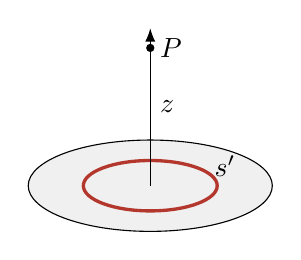
\begin{tikzpicture}[scale=1.0,>=Latex]
  \fill[black!6] (0,0) ellipse (1.55 and 0.58); \draw (0,0) ellipse (1.55 and 0.58);
  \draw[PosCharge,very thick] (0,0) ellipse (0.85 and 0.32); \node at (0.95,0.25) {$s'$};
  \draw[->] (0,0)--(0,2.0) node[midway,right] {$z$}; \fill (0,1.75) circle (1.5pt) node[right] {$P$};
\end{tikzpicture}
\end{minipage}\hfill
\begin{minipage}[c]{0.53\linewidth}
\[
dq=\sigma(2\pi s' ds'),
\qquad \text{skive}=\int_0^R\text{ring}.
\]
For $z>0$ og $V(\infty)=0$:
\[
\boxed{V(z)=\frac{\sigma}{2\varepsilon_0}\left(\sqrt{z^2+R^2}-z\right)}
\]
\[
\boxed{E_z(z)=\frac{\sigma}{2\varepsilon_0}\left(1-\frac{z}{\sqrt{z^2+R^2}}\right)}.
\]
\end{minipage}
\end{casebox}
\newpage
\section*{EV2 - Kuglegeometri: felt og potentiale \chaptertag{Kap. 2}}
\phantomsection
\addcontentsline{toc}{section}{EV2 - Find E/V: kugler, cylinder og plan}

\begin{casebox}{Massiv kugle: samme objekt, to Gauss-radier}
\begin{center}
\begin{minipage}[t]{0.48\linewidth}\centering
\textbf{$r<R$: inde}\\[1mm]
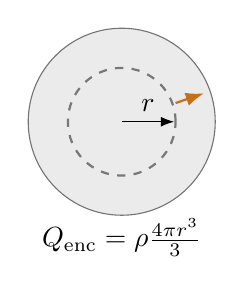
\begin{tikzpicture}[scale=0.95,>=Latex]
  \fill[black!8] (0,0) circle (1.25); \draw[black!55] (0,0) circle (1.25);
  \draw[dashed,GaussGray,thick] (0,0) circle (0.72);
  \draw[->] (0,0)--(0.70,0) node[midway,above] {$r$};
  \draw[->,Efield,thick] (0.72,0.25)--(1.10,0.38);
  \node at (0,-1.55) {$Q_{\rm enc}=\rho\frac{4\pi r^3}{3}$};
\end{tikzpicture}
\[
 E(4\pi r^2)=\frac{Q_{\rm enc}}{\varepsilon_0}
 \Rightarrow
 \boxed{\mathbf E=\frac{\rho r}{3\varepsilon_0}\hat r}.
\]
\[
 \boxed{V(r)=k\frac{Q}{2R}\left(3-\frac{r^2}{R^2}\right)}\quad(V(\infty)=0).
\]
\end{minipage}\hfill
\begin{minipage}[t]{0.48\linewidth}\centering
\textbf{$r>R$: ude}\\[1mm]
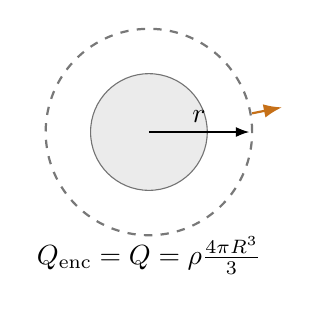
\begin{tikzpicture}[scale=0.95,>=Latex]
  \fill[black!8] (0,0) circle (0.78); \draw[black!55] (0,0) circle (0.78);
  \draw[dashed,GaussGray,thick] (0,0) circle (1.38);
  \draw[->] (0,0)--(1.34,0) node[midway,above] {$r$};
  \draw[->,Efield,thick] (1.38,0.25)--(1.78,0.33);
  \node at (0,-1.65) {$Q_{\rm enc}=Q=\rho\frac{4\pi R^3}{3}$};
\end{tikzpicture}
\[
 \boxed{\mathbf E=k\frac{Q}{r^2}\hat r}.
\]
\[
 \boxed{V(r)=k\frac{Q}{r}}.
\]
\end{minipage}
\end{center}
\casepitfall{$R$ er kuglens fysiske radius; $r$ er den variable Gauss-radius.}
\end{casebox}

\begin{casebox}{Tynd kugleskal: nul indenfor, punktladningsfelt udenfor}
\begin{center}
\begin{minipage}[t]{0.48\linewidth}\centering
\textbf{$r<R$}\\[1mm]
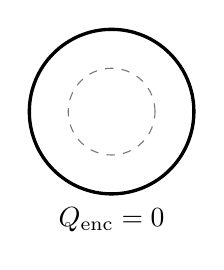
\begin{tikzpicture}[scale=0.95,>=Latex]
  \draw[very thick] (0,0) circle (1.1); \draw[dashed,GaussGray] (0,0) circle (0.58);
  \node at (0,-1.45) {$Q_{\rm enc}=0$};
\end{tikzpicture}
\[
 \boxed{\mathbf E=0}.\qquad\boxed{V=kQ/R}.
\]
\end{minipage}\hfill
\begin{minipage}[t]{0.48\linewidth}\centering
\textbf{$r>R$}\\[1mm]
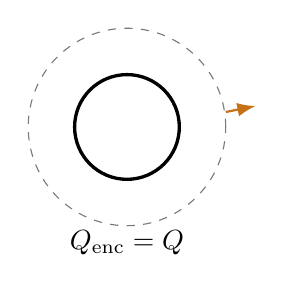
\begin{tikzpicture}[scale=0.95,>=Latex]
  \draw[very thick] (0,0) circle (0.7); \draw[dashed,GaussGray] (0,0) circle (1.32);
  \draw[->,Efield,thick] (1.32,0.2)--(1.72,0.28);
  \node at (0,-1.55) {$Q_{\rm enc}=Q$};
\end{tikzpicture}
\[
 \boxed{\mathbf E=k\frac{Q}{r^2}\hat r}.\qquad\boxed{V=kQ/r}.
\]
\end{minipage}
\end{center}
\end{casebox}

\begin{quickbox}{Gauss-startformel}
\[
 \boxed{\oint_S\mathbf E\cdot d\mathbf a=\frac{Q_{\rm enc}}{\varepsilon_0}}.
\]
Symmetri bestemmer både feltretningen og den del af Gauss-fladen, hvor $E$ er konstant.
\end{quickbox}

% ============================================================
\newpage
\section*{EV2 - Cylinder, linje og plan \chaptertag{Kap. 2}}

\begin{casebox}{Uniform massiv cylinder, radius $R$}
\begin{center}
\begin{minipage}[t]{0.48\linewidth}\centering
\textbf{$s<R$}\\[1mm]
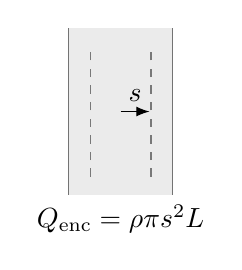
\begin{tikzpicture}[scale=0.92,>=Latex]
  \fill[black!8] (-0.72,-1.15) rectangle (0.72,1.15);
  \draw[black!55] (-0.72,-1.15)--(-0.72,1.15); \draw[black!55] (0.72,-1.15)--(0.72,1.15);
  \draw[dashed,GaussGray] (-0.42,-0.90)--(-0.42,0.90); \draw[dashed,GaussGray] (0.42,-0.90)--(0.42,0.90);
  \draw[->] (0,0)--(0.40,0) node[midway,above] {$s$};
  \node at (0,-1.48) {$Q_{\rm enc}=\rho\pi s^2L$};
\end{tikzpicture}
\[
 \boxed{\mathbf E=\frac{\rho s}{2\varepsilon_0}\hat s}.
\]
\end{minipage}\hfill
\begin{minipage}[t]{0.48\linewidth}\centering
\textbf{$s>R$}\\[1mm]
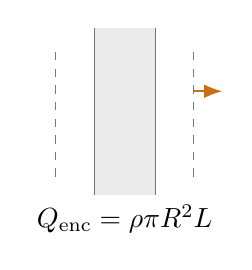
\begin{tikzpicture}[scale=0.92,>=Latex]
  \fill[black!8] (-0.42,-1.15) rectangle (0.42,1.15);
  \draw[black!55] (-0.42,-1.15)--(-0.42,1.15); \draw[black!55] (0.42,-1.15)--(0.42,1.15);
  \draw[dashed,GaussGray] (-0.95,-0.90)--(-0.95,0.90); \draw[dashed,GaussGray] (0.95,-0.90)--(0.95,0.90);
  \draw[->,Efield,thick] (0.95,0.28)--(1.35,0.28);
  \node at (0,-1.48) {$Q_{\rm enc}=\rho\pi R^2L$};
\end{tikzpicture}
\[
 \boxed{\mathbf E=\frac{\rho R^2}{2\varepsilon_0s}\hat s}.
\]
\end{minipage}
\end{center}
\end{casebox}

\begin{casebox}{Uendelig linjeladning}
\begin{minipage}[c]{0.43\linewidth}\centering
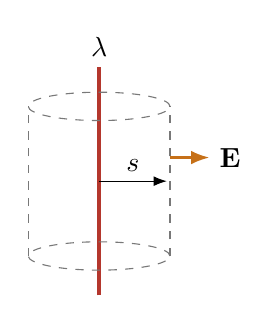
\begin{tikzpicture}[scale=1.0,>=Latex]
  \draw[very thick,PosCharge] (0,-1.45)--(0,1.45) node[above,text=black] {$\lambda$};
  \draw[dashed,GaussGray] (-0.90,-0.95)--(-0.90,0.95); \draw[dashed,GaussGray] (0.90,-0.95)--(0.90,0.95);
  \draw[dashed,GaussGray] (0,0.95) ellipse (0.90 and 0.18); \draw[dashed,GaussGray] (0,-0.95) ellipse (0.90 and 0.18);
  \draw[->,Efield,thick] (0.90,0.3)--(1.40,0.3) node[right,text=black] {$\mathbf E$};
  \draw[->] (0,0)--(0.86,0) node[midway,above] {$s$};
\end{tikzpicture}
\end{minipage}\hfill
\begin{minipage}[c]{0.53\linewidth}
\[
 Q_{\rm enc}=\lambda L,
\qquad
 E(2\pi sL)=\frac{\lambda L}{\varepsilon_0}.
\]
\[
 \boxed{\mathbf E=\frac{\lambda}{2\pi\varepsilon_0s}\hat s}.
\]
\casemethod{koaksial cylinder; kun lateralfladen bidrager til fluxen.}
\end{minipage}
\end{casebox}

\begin{quickbox}{Ikke-uniform cylindrisk ladning $\rho=\rho(s)$}
\[
\boxed{Q_{\rm enc}(s)=\int_0^s\rho(s')\\,2\pi s'L\\,ds'}
\quad (s<R).
\]
Brug derefter $E(2\pi sL)=Q_{\rm enc}/\varepsilon_0$. Man må ikke indsætte en standardformel for uniform $\rho$.
\end{quickbox}

\begin{casebox}{Ét uendeligt plan og to modsat ladede planer}
\begin{center}
\begin{minipage}[t]{0.48\linewidth}\centering
\textbf{Ét plan}\\[1mm]
\begin{tikzpicture}[scale=0.92,>=Latex]
  \draw[thick] (-1.5,0)--(1.5,0) node[right] {$\sigma$};
  \draw[dashed,GaussGray] (-0.55,-0.72) rectangle (0.55,0.72);
  \draw[->,Efield,thick] (0,0.12)--(0,1.18); \draw[->,Efield,thick] (0,-0.12)--(0,-1.18);
\end{tikzpicture}
\[
 2EA=\frac{\sigma A}{\varepsilon_0}
 \Rightarrow
 \boxed{E=\frac{\sigma}{2\varepsilon_0}}.
\]
\end{minipage}\hfill
\begin{minipage}[t]{0.48\linewidth}\centering
\textbf{To modsat ladede planer}\\[1mm]
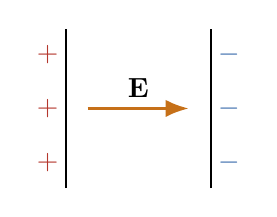
\begin{tikzpicture}[scale=0.92,>=Latex]
  \draw[thick] (-1.0,-1.1)--(-1.0,1.1); \draw[thick] (1.0,-1.1)--(1.0,1.1);
  \node[PosCharge] at (-1.25,0.75) {$+$}; \node[PosCharge] at (-1.25,0) {$+$}; \node[PosCharge] at (-1.25,-0.75) {$+$};
  \node[NegCharge] at (1.25,0.75) {$-$}; \node[NegCharge] at (1.25,0) {$-$}; \node[NegCharge] at (1.25,-0.75) {$-$};
  \draw[->,Efield,very thick] (-0.70,0)--(0.70,0) node[midway,above,text=black] {$\mathbf E$};
\end{tikzpicture}
\[
 \boxed{E_{\rm mellem}=\frac{\sigma}{\varepsilon_0}},\qquad
 \boxed{E_{\rm udenfor}=0}.
\]
For uendelige planer bruges potentialeforskelle: $\Delta V=-\int\mathbf E\cdot d\mathbf l$; $V(\infty)=0$ kan ikke bruges som reference.
\end{minipage}
\end{center}
\end{casebox}

% ============================================================
\newpage
\section*{EV3 - Region-for-region-problemer \chaptertag{Kap. 2}}
\phantomsection
\addcontentsline{toc}{section}{EV3 - Region-for-region}

\begin{quickbox}{Fast idé}
\[
 \boxed{\text{fysiske grænser }a,b,c,\ldots\text{ er faste}}
 \qquad
 \boxed{r\text{ eller }s\text{ er den variable Gauss-radius}}.
\]
\end{quickbox}

\begin{casebox}{Hul cylinder med uniform volumenladning i $a<s<b$}
\begin{center}
\begin{minipage}[t]{0.32\linewidth}\centering
\textbf{$s<a$}\\[1mm]
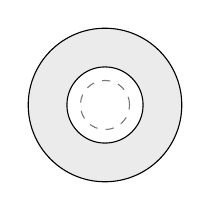
\begin{tikzpicture}[scale=0.78]
  \fill[black!8,even odd rule] (0,0) circle (1.25) (0,0) circle (0.62);
  \draw (0,0) circle (0.62); \draw (0,0) circle (1.25); \draw[dashed,GaussGray] (0,0) circle (0.40);
\end{tikzpicture}
\[
 Q_{\rm enc}=0,\qquad \boxed{E=0}.
\]
\end{minipage}
\begin{minipage}[t]{0.32\linewidth}\centering
\textbf{$a<s<b$}\\[1mm]
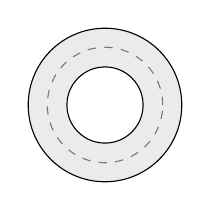
\begin{tikzpicture}[scale=0.78]
  \fill[black!8,even odd rule] (0,0) circle (1.25) (0,0) circle (0.62);
  \draw (0,0) circle (0.62); \draw (0,0) circle (1.25); \draw[dashed,GaussGray] (0,0) circle (0.94);
\end{tikzpicture}
\[
 Q_{\rm enc}=\rho\pi(s^2-a^2)L,
\]
\[
 \boxed{E=\frac{\rho(s^2-a^2)}{2\varepsilon_0s}}.
\]
\end{minipage}
\begin{minipage}[t]{0.32\linewidth}\centering
\textbf{$s>b$}\\[1mm]
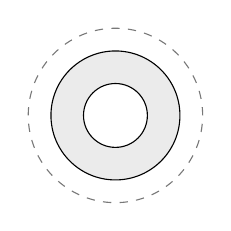
\begin{tikzpicture}[scale=0.78]
  \fill[black!8,even odd rule] (0,0) circle (1.05) (0,0) circle (0.52);
  \draw (0,0) circle (0.52); \draw (0,0) circle (1.05); \draw[dashed,GaussGray] (0,0) circle (1.42);
\end{tikzpicture}
\[
 Q_{\rm enc}=\rho\pi(b^2-a^2)L,
\]
\[
 \boxed{E=\frac{\rho(b^2-a^2)}{2\varepsilon_0s}}.
\]
\end{minipage}
\end{center}
\end{casebox}

\begin{casebox}{Koncentriske radier: læs geometrien som et regionskort}
\begin{minipage}[c]{0.45\linewidth}\centering
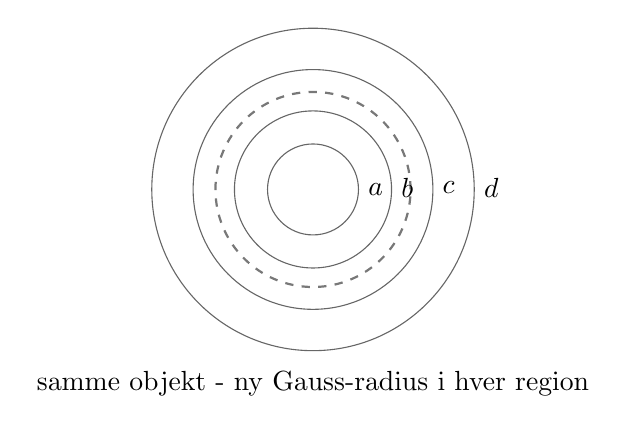
\begin{tikzpicture}[scale=1.05,>=Latex]
  \foreach \r in {0.55,0.95,1.45,1.95}{\draw[black!60] (0,0) circle (\r);}
  \draw[dashed,GaussGray,thick] (0,0) circle (1.18);
  \node[right] at (0.55,0) {$a$}; \node[right] at (0.95,0.02) {$b$}; \node[right] at (1.45,0.02) {$c$}; \node[right] at (1.95,0.02) {$d$};
  \node at (0,-2.35) {samme objekt - ny Gauss-radius i hver region};
\end{tikzpicture}
\end{minipage}\hfill
\begin{minipage}[c]{0.51\linewidth}
\[
 r<a,\quad a<r<b,\quad b<r<c,\quad c<r<d,\quad r>d.
\]
\[
 \boxed{\text{vælg region}\to Q_{\rm enc}(r)\to\text{Gauss}\to E(r)}.
\]
\casepitfall{man trækker ikke felterne ved to grænser fra hinanden; feltet i regionen findes direkte fra den omsluttede ladning.}
\end{minipage}
\end{casebox}

% ============================================================
\newpage
\begin{casebox}{Hul / boring i en ladningsfordeling: superposition}
\begin{minipage}[c]{0.48\linewidth}\centering
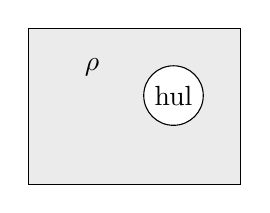
\begin{tikzpicture}[scale=0.9]
  \fill[black!8] (-1.5,-1.1) rectangle (1.5,1.1); \draw (-1.5,-1.1) rectangle (1.5,1.1);
  \fill[white] (0.55,0.15) circle (0.42); \draw (0.55,0.15) circle (0.42); \node at (-0.6,0.55) {$\rho$};
  \node at (0.55,0.15) {hul};
\end{tikzpicture}
\end{minipage}\hfill
\begin{minipage}[c]{0.48\linewidth}
\[
\boxed{\text{fysisk hul}=\text{fuld fordeling }(+\rho)+\text{ hjælpefordeling }(-\rho)}.
\]
\[
\boxed{\mathbf E_{\rm hul}=\mathbf E_{+\rho}+\mathbf E_{-\rho}}.
\]
\casemethod{løs de to simple fordelinger hver for sig med samme koordinatsystem og læg felterne vektorielt sammen.}
\end{minipage}
\end{casebox}

\newpage
\section*{EV4 - Ledere og hulrum \chaptertag{Kap. 2 + 4}}
\phantomsection
\addcontentsline{toc}{section}{EV4 - Ledere og hulrum}

\begin{casebox}{Perfekt leder i elektrostatisk ligevægt}
\begin{minipage}[c]{0.44\linewidth}\centering
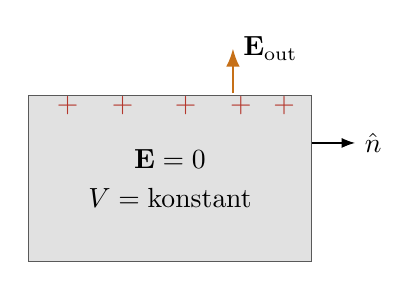
\begin{tikzpicture}[scale=1.0,>=Latex]
  \fill[ConductorGray] (-1.8,-1.05) rectangle (1.8,1.05); \draw[black!65] (-1.8,-1.05) rectangle (1.8,1.05);
  \node at (0,0.25) {$\mathbf E=0$}; \node at (0,-0.25) {$V=\text{konstant}$};
  \foreach \x in {-1.3,-0.6,0.2,0.9,1.45}{\node[PosCharge] at (\x,0.93) {$+$};}
  \draw[->,Efield,thick] (0.8,1.08)--(0.8,1.65) node[right,text=black] {$\mathbf E_{\rm out}$};
  \draw[->] (1.8,0.45)--(2.35,0.45) node[right] {$\hat n$};
\end{tikzpicture}
\end{minipage}\hfill
\begin{minipage}[c]{0.52\linewidth}
\[
 \boxed{\mathbf E=0\text{ i metallet}},\qquad
 \boxed{V=\text{konstant}},\qquad
 \boxed{\rho=0\text{ i bulk}}.
\]
\[
 \boxed{\mathbf E_{\rm out}=\frac{\sigma}{\varepsilon_0}\hat n},\qquad E_{\parallel}=0.
\]
\casemethod{ladning i en leder ender på overfladerne; en Gauss-flade inde i metal omslutter netto nul ladning.}
\end{minipage}
\end{casebox}

\begin{casebox}{Ekstern ladning nær neutral leder: induktion}
\begin{minipage}[c]{0.50\linewidth}\centering
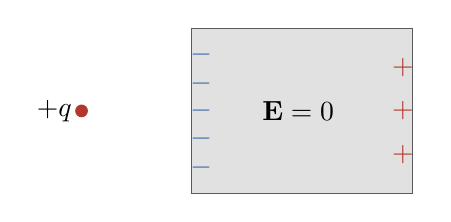
\begin{tikzpicture}[scale=1.0,>=Latex]
  \fill[PosCharge] (-2.2,0) circle (2.3pt) node[left,text=black] {$+q$};
  \fill[ConductorGray] (-0.8,-1.05) rectangle (2.0,1.05); \draw[black!65] (-0.8,-1.05) rectangle (2.0,1.05);
  \foreach \y in {-0.72,-0.35,0,0.35,0.72}{\node[NegCharge] at (-0.68,\y) {$-$};}
  \foreach \y in {-0.55,0,0.55}{\node[PosCharge] at (1.88,\y) {$+$};}
  \node at (0.55,0) {$\mathbf E=0$};
\end{tikzpicture}
\end{minipage}\hfill
\begin{minipage}[c]{0.46\linewidth}
\textbf{Genkend:} ekstern ladning polariserer lederens overfladeladning.
\[
 \mathbf E=0\quad\text{i selve metallet}.
\]
\casemethod{brug lederbetingelser + symmetri/spejlingsmetode, hvis geometrien tillader det.}
\casepitfall{den inducerede $\sigma$ er normalt ikke uniform.}
\end{minipage}
\end{casebox}

\begin{casebox}{Tomt lukket hulrum i leder}
\begin{minipage}[c]{0.45\linewidth}\centering
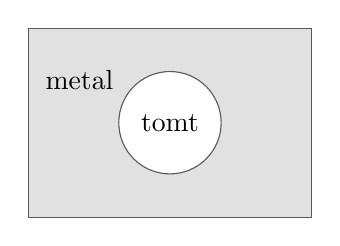
\begin{tikzpicture}[scale=1.0]
  \fill[ConductorGray] (-1.8,-1.2) rectangle (1.8,1.2); \fill[white] (0,0) circle (0.65);
  \draw[black!65] (-1.8,-1.2) rectangle (1.8,1.2); \draw[black!65] (0,0) circle (0.65);
  \node at (0,0) {tomt}; \node at (-1.15,0.55) {metal};
\end{tikzpicture}
\end{minipage}\hfill
\begin{minipage}[c]{0.51\linewidth}
\[
 Q_{\rm hulrum}=0,\qquad V=\text{konstant på randen}
\]
\[
 \boxed{\mathbf E=0\text{ i det lukkede tomme hulrum}}.
\]
\textbf{Faraday-cage-logik:} statiske ydre felter trænger ikke ind i et lukket tomt hulrum i en ideel leder.
\end{minipage}
\end{casebox}

% ============================================================
\newpage
\section*{EV4 - Ladning i hulrum og koncentriske ledere \chaptertag{Kap. 2 + 4}}

\begin{casebox}{Ladning $q$ i hulrum: femtrinsargumentet}
\begin{center}
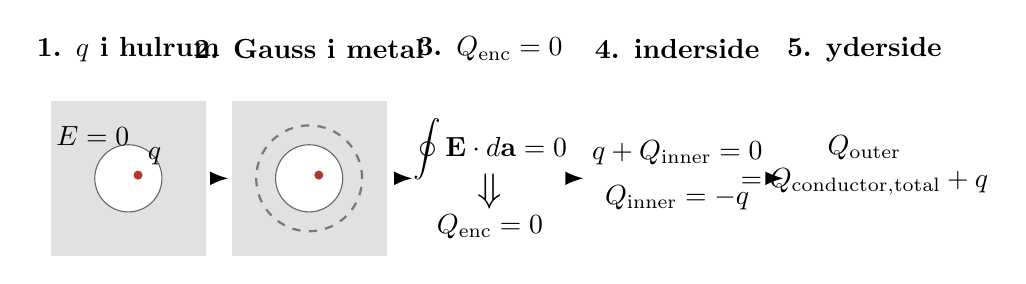
\begin{tikzpicture}[>=Latex,scale=0.82]
  \node[font=\bfseries] at (-5.6,2.0) {1. $q$ i hulrum};
  \fill[ConductorGray] (-6.8,-1.2) rectangle (-4.4,1.2); \fill[white] (-5.6,0) circle (0.52); \draw[black!60] (-5.6,0) circle (0.52);
  \fill[PosCharge] (-5.45,0.05) circle (2.0pt) node[above right,text=black] {$q$};
  \node at (-6.15,0.65) {$E=0$};
  \node[font=\bfseries] at (-2.8,2.0) {2. Gauss i metal};
  \fill[ConductorGray] (-4.0,-1.2) rectangle (-1.6,1.2); \fill[white] (-2.8,0) circle (0.52); \draw[black!60] (-2.8,0) circle (0.52);
  \fill[PosCharge] (-2.65,0.05) circle (2.0pt); \draw[dashed,GaussGray,thick] (-2.8,0) circle (0.82);
  \node[font=\bfseries] at (0,2.0) {3. $Q_{\rm enc}=0$};
  \node at (0,0.45) {$\displaystyle\oint\mathbf E\cdot d\mathbf a=0$}; \node[font=\Large] at (0,-0.2) {$\Downarrow$}; \node at (0,-0.75) {$Q_{\rm enc}=0$};
  \node[font=\bfseries] at (2.9,2.0) {4. inderside};
  \node at (2.9,0.4) {$q+Q_{\rm inner}=0$}; \node[font=\bfseries] at (2.9,-0.3) {$Q_{\rm inner}=-q$};
  \node[font=\bfseries] at (5.8,2.0) {5. yderside};
  \node[align=center] at (5.8,0.2) {$Q_{\rm outer}$\\$=Q_{\rm conductor,total}+q$};
  \draw[->,thick] (-4.25,0)--(-4.05,0); \draw[->,thick] (-1.4,0)--(-1.2,0); \draw[->,thick] (1.25,0)--(1.45,0); \draw[->,thick] (4.35,0)--(4.55,0);
\end{tikzpicture}
\end{center}
\casepitfall{Gauss bestemmer total indre ladning. Uden ekstra symmetri behøver den lokale $\sigma$ ikke være uniform.}
\end{casebox}

\begin{casebox}{Koncentriske ledere: fire fysiske overflader}
\begin{minipage}[c]{0.44\linewidth}\centering
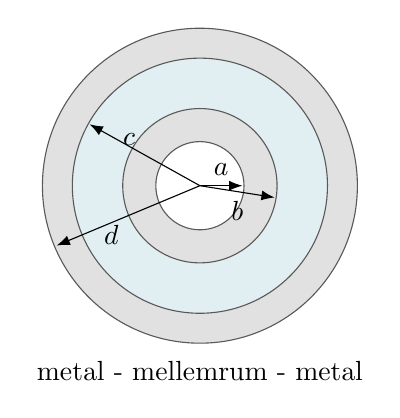
\begin{tikzpicture}[scale=1.0,>=Latex]
  \fill[ConductorGray,even odd rule] (0,0) circle (2.0) (0,0) circle (1.62);
  \fill[DielectricTint,even odd rule] (0,0) circle (1.62) (0,0) circle (0.98);
  \fill[ConductorGray,even odd rule] (0,0) circle (0.98) (0,0) circle (0.56);
  \foreach \r in {0.56,0.98,1.62,2.0}{\draw[black!65] (0,0) circle (\r);}
  \draw[->] (0,0)--(0.54,0) node[midway,above] {$a$}; \draw[->] (0,0)--(0.95,-0.15) node[midway,below] {$b$};
  \draw[->] (0,0)--(-1.40,0.78) node[midway,above left] {$c$}; \draw[->] (0,0)--(-1.82,-0.76) node[midway,below left] {$d$};
  \node at (0,-2.35) {metal - mellemrum - metal};
\end{tikzpicture}
\end{minipage}\hfill
\begin{minipage}[c]{0.52\linewidth}
\[
 \boxed{Q_a=0,\quad Q_b=Q_1,\quad Q_c=-Q_1,\quad Q_d=Q_1+Q_2}.
\]
\[
 \sigma_b=\frac{Q_1}{4\pi b^2},\quad
 \sigma_c=-\frac{Q_1}{4\pi c^2},\quad
 \sigma_d=\frac{Q_1+Q_2}{4\pi d^2}.
\]
\casemethod{gå én fysisk overflade ad gangen: Gauss i metal $\to Q_{\rm enc}=0$; brug derefter hver leders givne nettoladning.}
\end{minipage}
\end{casebox}

\begin{casebox}{Cylindrisk eksamenscase F22.2}
\begin{minipage}[c]{0.42\linewidth}\centering
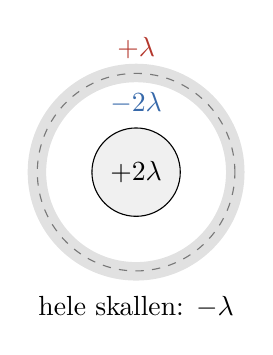
\begin{tikzpicture}[scale=1.02]
  \filldraw[fill=black!6] (0,0) circle (0.55);
  \fill[ConductorGray,even odd rule] (0,0) circle (1.35) (0,0) circle (1.12);
  \draw[dashed,GaussGray] (0,0) circle (1.23);
  \node at (0,0) {$+2\lambda$}; \node[NegCharge] at (0,0.86) {$-2\lambda$}; \node[PosCharge] at (0,1.55) {$+\lambda$};
  \node at (0,-1.68) {hele skallen: $-\lambda$};
\end{tikzpicture}
\end{minipage}\hfill
\begin{minipage}[c]{0.54\linewidth}
\[
 2\lambda+\lambda_{\rm inner}=0\Rightarrow \boxed{\lambda_{\rm inner}=-2\lambda},
\]
\[
 \lambda_{\rm inner}+\lambda_{\rm outer}=-\lambda\Rightarrow \boxed{\lambda_{\rm outer}=+\lambda}.
\]
Mellem stang og skal, $a<s<b$:
\[
 \boxed{\mathbf E(s)=\frac{\lambda}{\pi\varepsilon_0s}\hat s}.
\]
\casepitfall{$-\lambda$ er hele skallens totale ladning, ikke ydersidens ladning.}
\end{minipage}
\end{casebox}

% ============================================================
\newpage
\section*{EV5 - Randværdier: Poisson og Laplace \chaptertag{Kap. 3}}
\phantomsection
\addcontentsline{toc}{section}{EV5 - Randværdiproblemer: Poisson/Laplace}

\begin{quickbox}{Recognition: randværdiproblem}
\[
\boxed{\text{geometri + randbetingelser}\to V\to\mathbf E=-\nabla V}.
\]
Ladningsfrit område $\to$ Laplace. Kendt $\rho$ $\to$ Poisson. Punktladning nær jordet leder $\to$ overvej spejlingsmetoden.
\end{quickbox}
\begin{casebox}{Poisson: region med ladning}
\begin{minipage}[c]{0.42\linewidth}\centering
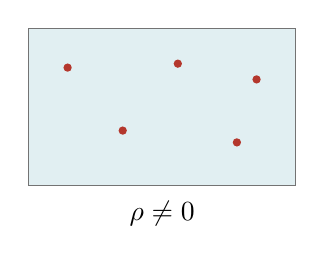
\begin{tikzpicture}[scale=1.0]
  \fill[DielectricTint] (-1.7,-1.0) rectangle (1.7,1.0); \draw[black!55] (-1.7,-1.0) rectangle (1.7,1.0);
  \foreach \x/\y in {-1.2/0.5,-0.5/-0.3,0.2/0.55,0.95/-0.45,1.2/0.35}{\fill[PosCharge] (\x,\y) circle (1.5pt);}
  \node at (0,-1.35) {$\rho\neq0$};
\end{tikzpicture}
\end{minipage}\hfill
\begin{minipage}[c]{0.54\linewidth}
\[
 \boxed{\nabla^2V=-\frac{\rho}{\varepsilon_0}}.
\]
\textbf{Brug når:} kilden $\rho$ er kendt og potentialet søges via differentialligningen.
\end{minipage}
\end{casebox}

\begin{casebox}{Laplace: ladningsfrit område bestemt af randen}
\begin{minipage}[c]{0.42\linewidth}\centering
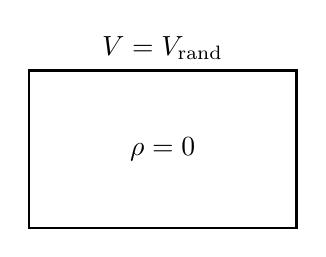
\begin{tikzpicture}[scale=1.0]
  \draw[thick] (-1.7,-1.0) rectangle (1.7,1.0); \node at (0,0) {$\rho=0$};
  \node at (0,1.28) {$V=V_{\rm rand}$};
\end{tikzpicture}
\end{minipage}\hfill
\begin{minipage}[c]{0.54\linewidth}
\[
 \boxed{\rho=0\Rightarrow\nabla^2V=0}.
\]
\[
 \boxed{\text{geometri}\to\text{koordinater}\to\text{separation}\to\text{randbetingelser}}.
\]
1D-specialtilfælde:
\[
 V=V(x)\Rightarrow \frac{d^2V}{dx^2}=0\Rightarrow \boxed{V=Ax+B}.
\]
\end{minipage}
\end{casebox}

\begin{casebox}{Kontrolcase: kan et foreslået felt være elektrostatisk?}
I et ladningsfrit elektrostatisk område skal begge gælde:
\[
 \boxed{\nabla\cdot\mathbf E=0},\qquad \boxed{\nabla\times\mathbf E=0}.
\]
Hvis potentialet er givet i samme område:
\[
 \boxed{\nabla^2V=0}.
\]
\end{casebox}

\begin{casebox}{Kartesisk separation}
\begin{minipage}[c]{0.44\linewidth}\centering
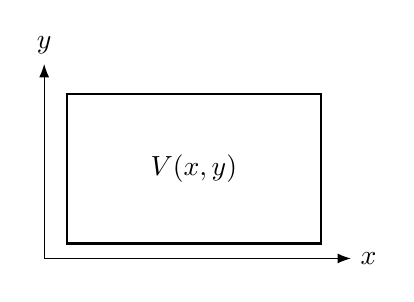
\begin{tikzpicture}[scale=0.95,>=Latex]
  \draw[thick] (-1.7,-1.0) rectangle (1.7,1.0); \draw[->] (-2.0,-1.2)--(2.1,-1.2) node[right] {$x$}; \draw[->] (-2.0,-1.2)--(-2.0,1.4) node[above] {$y$};
  \node at (0,0) {$V(x,y)$};
\end{tikzpicture}
\end{minipage}\hfill
\begin{minipage}[c]{0.52\linewidth}
\[
 \frac{\partial^2V}{\partial x^2}+\frac{\partial^2V}{\partial y^2}=0,\qquad V=X(x)Y(y).
\]
\[
 \frac{X''}{X}+\frac{Y''}{Y}=0.
\]
Et praktisk valg:
\[
 X''-k^2X=0,\qquad Y''+k^2Y=0,
\]
med eksponential/hyperbolsk hhv. trigonometrisk løsning.
\end{minipage}
\end{casebox}

% ============================================================
\newpage
\section*{EV5 - Separation i sfærisk geometri / Legendre \chaptertag{Kap. 3}}

\begin{casebox}{Sfærisk, aksialsymmetrisk Laplace}
\begin{minipage}[c]{0.40\linewidth}\centering
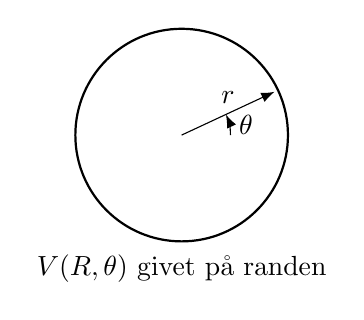
\begin{tikzpicture}[scale=1.0,>=Latex]
  \draw[thick] (0,0) circle (1.35); \draw[->] (0,0)--(1.18,0.55) node[midway,above] {$r$};
  \draw[->] (0.62,0) arc (0:25:0.62) node[midway,right] {$\theta$};
  \node at (0,-1.70) {$V(R,\theta)$ givet på randen};
\end{tikzpicture}
\end{minipage}\hfill
\begin{minipage}[c]{0.56\linewidth}
\[
 \boxed{V(r,\theta)=\sum_{\ell=0}^{\infty}\left(A_\ell r^\ell+\frac{B_\ell}{r^{\ell+1}}\right)P_\ell(\cos\theta)}.
\]
Indenfor inkl. $r=0$: behold $r^\ell$. Udenfor med $V(\infty)=0$: behold $r^{-(\ell+1)}$.
\[
 P_0=1,\quad P_1=x,\quad P_2=\tfrac12(3x^2-1),\quad P_3=\tfrac12(5x^3-3x).
\]
\casemethod{$V(R,\theta)\propto P_\ell(\cos\theta)$ $\Rightarrow$ kun samme $\ell$-led er nødvendigt.}
\end{minipage}
\end{casebox}

\begin{casebox}{J26.5-type: én Legendre-mode}
\[
 V(R,\theta)=2V_0P_2(\cos\theta)\Rightarrow \ell=2.
\]
\[
 V_{\rm inde}\propto r^2P_2(\cos\theta),\qquad V_{\rm ude}\propto r^{-3}P_2(\cos\theta).
\]
Fra $V$ til felt:
\[
 E_r=-\frac{\partial V}{\partial r},\qquad
 E_\theta=-\frac1r\frac{\partial V}{\partial\theta},\qquad E_\phi=0.
\]
\textbf{Gamle opgaver:} nov21.3, jan26.5.
\end{casebox}

% ============================================================
\newpage
\section*{EV5 - Spejlingsmetoden \chaptertag{Kap. 3}}
\phantomsection
\addcontentsline{toc}{section}{EV5 - Randværdiproblemer: spejlingsmetoden}

\begin{quickbox}{Entydighedsteorem - hvorfor spejling virker}
Når en konstrueret løsning opfylder den korrekte differentialligning og de givne randbetingelser, er løsningen i det fysiske område entydig.
\end{quickbox}
\begin{casebox}{Punktladning over jordet plan}
\begin{minipage}[c]{0.50\linewidth}\centering
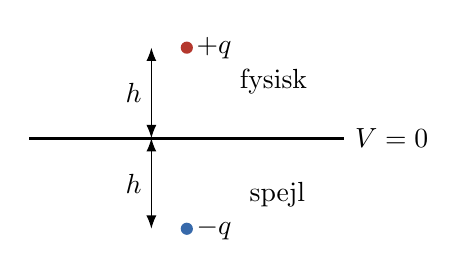
\begin{tikzpicture}[scale=1.0,>=Latex]
  \draw[very thick] (-2.0,0)--(2.0,0) node[right] {$V=0$};
  \fill[PosCharge] (0,1.15) circle (2.2pt) node[right,text=black] {$+q$};
  \fill[NegCharge] (0,-1.15) circle (2.2pt) node[right,text=black] {$-q$};
  \draw[<->] (-0.45,0)--(-0.45,1.15) node[midway,left] {$h$}; \draw[<->] (-0.45,0)--(-0.45,-1.15) node[midway,left] {$h$};
  \node at (1.15,-0.72) {spejl}; \node at (1.1,0.72) {fysisk};
\end{tikzpicture}
\end{minipage}\hfill
\begin{minipage}[c]{0.46\linewidth}
\[
 (x_0,h),+q\quad\longrightarrow\quad(x_0,-h),-q.
\]
\[
 \boxed{V=0\text{ på lederplanet}}.
\]
\[
 \boxed{\text{spejlladningen er ikke fysisk}}.
\]
\casemethod{erstat lederen med spejlladningen; brug derefter almindelig Coulomb/potentiale i det fysiske område.}
\end{minipage}
\end{casebox}

\begin{casebox}{To vinkelrette jordede planer}
\begin{minipage}[c]{0.46\linewidth}\centering
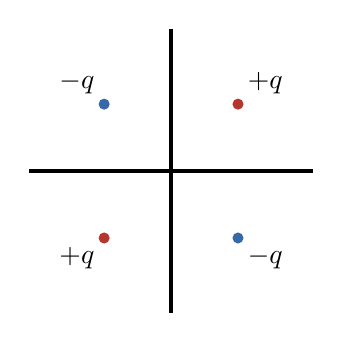
\begin{tikzpicture}[scale=1.0]
  \draw[very thick] (-1.8,0)--(1.8,0); \draw[very thick] (0,-1.8)--(0,1.8);
  \fill[PosCharge] (0.85,0.85) circle (2pt) node[above right,text=black] {$+q$};
  \fill[NegCharge] (-0.85,0.85) circle (2pt) node[above left,text=black] {$-q$};
  \fill[NegCharge] (0.85,-0.85) circle (2pt) node[below right,text=black] {$-q$};
  \fill[PosCharge] (-0.85,-0.85) circle (2pt) node[below left,text=black] {$+q$};
\end{tikzpicture}
\end{minipage}\hfill
\begin{minipage}[c]{0.50\linewidth}
Én spejling skifter fortegn; to spejlinger giver plus igen.
\[
 +q\to(-q)_x,\qquad +q\to(-q)_y,\qquad +q\to(+q)_{xy}.
\]
\casemethod{vælg spejle, så $V=0$ opfyldes på begge planer samtidig.}
\casepitfall{ingen selvkraft fra ladningen på sig selv; brug kun andre rigtige ladninger + relevante spejle.}
\end{minipage}
\textbf{Gamle opgaver:} nov24.1, nov25.1.
\end{casebox}

% ============================================================
\newpage
\section*{EV6 - Multipoler og fjernfelt \chaptertag{Kap. 3}}
\begin{quickbox}{Recognition}
\[
\boxed{r\gg\text{ladningsfordelingens størrelse}\to\text{overvej multipolekspansion}}.
\]
\end{quickbox}
\phantomsection
\addcontentsline{toc}{section}{EV6 - Multipoler og fjernfelt}

\begin{center}
\begin{minipage}[t]{0.31\linewidth}
\begin{casebox}{Monopol}
\begin{center}
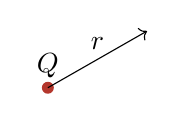
\begin{tikzpicture}[scale=0.9]
  \fill[PosCharge] (0,0) circle (2.4pt) node[above,text=black] {$Q$}; \draw[->] (0,0)--(1.4,0.8) node[midway,above] {$r$};
\end{tikzpicture}
\end{center}
\[
 V_{\rm mon}=k\frac{Q}{r},\qquad V\sim r^{-1}.
\]
\end{casebox}
\end{minipage}\hfill
\begin{minipage}[t]{0.31\linewidth}
\begin{casebox}{Dipol}
\begin{center}
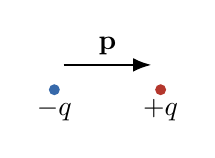
\begin{tikzpicture}[scale=0.9,>=Latex]
  \fill[NegCharge] (-0.75,0) circle (2.2pt) node[below,text=black] {$-q$}; \fill[PosCharge] (0.75,0) circle (2.2pt) node[below,text=black] {$+q$};
  \draw[->,thick] (-0.62,0.35)--(0.62,0.35) node[midway,above] {$\mathbf p$};
\end{tikzpicture}
\end{center}
\[
 \mathbf p=q\mathbf d,
\]
\[
 V_{\rm dip}=k\frac{\mathbf p\cdot\hat r}{r^2},\qquad V\sim r^{-2}.
\]
\end{casebox}
\end{minipage}\hfill
\begin{minipage}[t]{0.31\linewidth}
\begin{casebox}{Quadrupol}
\begin{center}
\begin{tikzpicture}[scale=0.85]
  \fill[PosCharge] (-0.8,0.6) circle (2pt); \fill[PosCharge] (0.8,-0.6) circle (2pt); \fill[NegCharge] (0.8,0.6) circle (2pt); \fill[NegCharge] (-0.8,-0.6) circle (2pt);
  \node[PosCharge] at (-1.1,0.6) {$+$}; \node[PosCharge] at (1.1,-0.6) {$+$}; \node[NegCharge] at (1.1,0.6) {$-$}; \node[NegCharge] at (-1.1,-0.6) {$-$};
\end{tikzpicture}
\end{center}
\[
 Q=0,\quad \mathbf p=0,
\]
\[
 V_{\rm quad}\sim r^{-3}.
\]
\end{casebox}
\end{minipage}
\end{center}

\begin{quickbox}{Fjernfelthierarki}
\[
 \boxed{V_{\rm mon}\sim r^{-1},\qquad V_{\rm dip}\sim r^{-2},\qquad V_{\rm quad}\sim r^{-3}}.
\]
\[
 Q\neq0\Rightarrow\text{monopol};\qquad Q=0,\mathbf p\neq0\Rightarrow\text{dipol};\qquad Q=0,\mathbf p=0\Rightarrow\text{undersøg quadrupol}.
\]
\end{quickbox}

\begin{casebox}{Generel dipol og Griffiths-multipoludvikling}
\[
 \mathbf p=\sum_iq_i\mathbf r_i=\iiint\mathbf r'\rho(\mathbf r')\,d\tau'.
\]
For $\mathbf p=p\hat z$:
\[
 V_{\rm dip}=k\frac{p\cos\theta}{r^2},\qquad
 \mathbf E_{\rm dip}=k\frac{p}{r^3}(2\cos\theta\,\hat r+\sin\theta\,\hat\theta).
\]
Generelt, $r>r'$:
\[
 V(\mathbf r)=k\sum_{\ell=0}^{\infty}\frac{1}{r^{\ell+1}}\iiint (r')^\ell P_\ell(\cos\alpha)\rho(\mathbf r')\,d\tau'.
\]
\end{casebox}

\begin{casebox}{F23.3-type: se annullationerne i fjernfeltet}
\[
 Q=0,\qquad p_z=0\qquad\Rightarrow\qquad\text{første ikke-nul led er quadrupol}.
\]
På $+z$-aksen:
\[
 \mathbf E(z)=\frac{q}{4\pi\varepsilon_0}\left[\frac1{(z-d)^2}+\frac1{(z+d)^2}-\frac{2}{z^2}\right]\hat z.
\]
For $d/z\ll1$ overlever anden orden:
\[
 \boxed{\mathbf E(z)=\frac{6qd^2}{4\pi\varepsilon_0z^4}\hat z}.
\]
Hvis $\Theta=2qd^2$: $\mathbf E=3\Theta/(4\pi\varepsilon_0z^4)\hat z$.\
\textbf{Gamle opgaver:} feb22.1, feb23.3, jan26.1.
\end{casebox}

% ============================================================
\newpage
\section*{EV7 - Elektriske materialer: polarisation \chaptertag{Kap. 4}}
\phantomsection
\addcontentsline{toc}{section}{EV7 - Elektriske materialer}

\begin{casebox}{Polarisation: før og efter ydre felt}
\begin{center}
\begin{minipage}[t]{0.48\linewidth}\centering
\textbf{Uden ydre felt}\\[1mm]
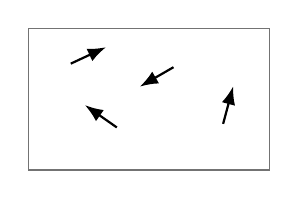
\begin{tikzpicture}[scale=0.9,>=Latex]
  \draw[black!55] (-1.7,-1.0) rectangle (1.7,1.0);
  \foreach \x/\y/\a in {-1.1/0.5/25,-0.45/-0.4/145,0.35/0.45/210,1.05/-0.35/75}{\draw[->,thick] (\x,\y)--++({0.55*cos(\a)},{0.55*sin(\a)});}
\end{tikzpicture}
\end{minipage}\hfill
\begin{minipage}[t]{0.48\linewidth}\centering
\textbf{Ydre $\mathbf E$}\\[1mm]
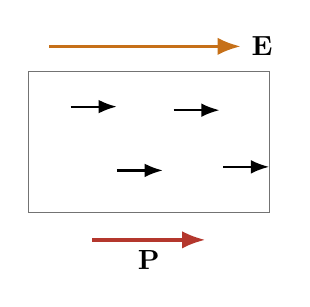
\begin{tikzpicture}[scale=0.9,>=Latex]
  \draw[black!55] (-1.7,-1.0) rectangle (1.7,1.0); \draw[->,Efield,very thick] (-1.4,1.35)--(1.3,1.35) node[right,text=black] {$\mathbf E$};
  \foreach \x/\y in {-1.1/0.5,-0.45/-0.4,0.35/0.45,1.05/-0.35}{\draw[->,thick] (\x,\y)--++(0.65,0);}
  \draw[->,PosCharge,very thick] (-0.8,-1.38)--(0.8,-1.38) node[midway,below,text=black] {$\mathbf P$};
\end{tikzpicture}
\end{minipage}
\end{center}
\[
 \boxed{\mathbf P=\frac{d\mathbf p}{d\tau}}\qquad\text{(dipolmoment pr. volumen)}.
\]
\end{casebox}

\begin{casebox}{Bundne ladninger fra $\mathbf P$}
\begin{minipage}[c]{0.44\linewidth}\centering
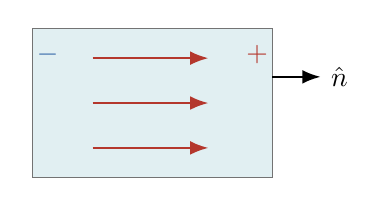
\begin{tikzpicture}[scale=0.95,>=Latex]
  \fill[DielectricTint] (-1.6,-1.0) rectangle (1.6,1.0); \draw[black!55] (-1.6,-1.0) rectangle (1.6,1.0);
  \foreach \y in {-0.6,0,0.6}{\draw[->,PosCharge,thick] (-0.8,\y)--(0.75,\y);}
  \draw[->,thick] (1.6,0.35)--(2.25,0.35) node[right] {$\hat n$};
  \node[NegCharge] at (-1.4,0.65) {$-$}; \node[PosCharge] at (1.4,0.65) {$+$};
\end{tikzpicture}
\end{minipage}\hfill
\begin{minipage}[c]{0.52\linewidth}
\[
 \boxed{\rho_b=-\nabla\cdot\mathbf P},\qquad
 \boxed{\sigma_b=\mathbf P\cdot\hat n}.
\]
\[
 Q_b^{\rm vol}=\iiint\rho_b\,d\tau,\qquad Q_b^{\rm surf}=\iint\sigma_b\,da.
\]
\casemethod{beregn først divergensen; evaluer derefter $\mathbf P\cdot\hat n$ separat på hver fysisk overflade.}
\casepitfall{tæthed er ikke total ladning.}
\end{minipage}
\end{casebox}

\begin{casebox}{F24.2-type: $\mathbf P=A(x\hat x+y\hat y+z\hat z)$ i kube}
\[
 \rho_b=-\nabla\cdot\mathbf P=-3A.
\]
På fx $x=L/2$, $\hat n=\hat x$:
\[
 \sigma_b=\mathbf P\cdot\hat n=Ax=\boxed{AL/2}.
\]
Samme resultat på alle seks flader; kontrol:
\[
 Q_b^{\rm vol}=-3AL^3,\qquad Q_b^{\rm surf}=+3AL^3\Rightarrow Q_b^{\rm total}=0.
\]
\casepitfall{$L/2$ er fladens koordinat, ikke dens areal.}
\end{casebox}

% ============================================================
\newpage
\section*{EV7 - $\mathbf D$-felt og lineære dielektrika \chaptertag{Kap. 4}}

\begin{casebox}{$\mathbf D$: brug kun den frie ladning}
\begin{minipage}[c]{0.44\linewidth}\centering
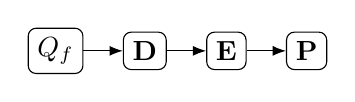
\begin{tikzpicture}[scale=0.95,>=Latex,node distance=5mm]
  \node[draw,rounded corners=1mm] (q) {$Q_f$}; \node[draw,rounded corners=1mm,right=of q] (d) {$\mathbf D$}; \node[draw,rounded corners=1mm,right=of d] (e) {$\mathbf E$}; \node[draw,rounded corners=1mm,right=of e] (p) {$\mathbf P$};
  \draw[->] (q)--(d); \draw[->] (d)--(e); \draw[->] (e)--(p);
\end{tikzpicture}
\end{minipage}\hfill
\begin{minipage}[c]{0.52\linewidth}
\[
 \boxed{\mathbf D=\varepsilon_0\mathbf E+\mathbf P},\qquad
 \boxed{\nabla\cdot\mathbf D=\rho_f},
\]
\[
 \boxed{\oint\mathbf D\cdot d\mathbf a=Q_{f,\rm enc}}.
\]
Ved lederoverflade:
\[
 (\mathbf D_{\rm ude}-\mathbf D_{\rm inde})\cdot\hat n=\sigma_f.
\]
\end{minipage}
\end{casebox}

\begin{casebox}{Lineært homogent dielektrikum}
\[
 \boxed{\mathbf P=\varepsilon_0\chi_e\mathbf E},\qquad
 \boxed{\mathbf D=\varepsilon\mathbf E=\varepsilon_0\varepsilon_r\mathbf E},
\]
\[
 \varepsilon=\varepsilon_0\varepsilon_r,\qquad \chi_e=\varepsilon_r-1.
\]
\casemethod{$Q_f\to\mathbf D\to\mathbf E\to\mathbf P\to\rho_b,\sigma_b$.}
\end{casebox}
\begin{quickbox}{Samme geometri som tidligere - nu med materiale}
Kugle, cylinder og plan løses stadig med symmetri. Forskellen er, at $\oint\mathbf D\cdot d\mathbf a=Q_{f,\rm enc}$ bruger den frie ladning; derefter findes $\mathbf E$ fra materialerelationen.
\[
\boxed{Q_{f,\rm enc}\to\mathbf D\to\mathbf E\to V}.
\]
\end{quickbox}

\begin{casebox}{N23.4-type: lederkugle mellem to dielektrika}
\begin{minipage}[c]{0.43\linewidth}\centering
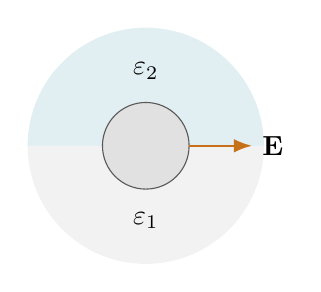
\begin{tikzpicture}[scale=1.0,>=Latex]
  \fill[DielectricTint] (-1.5,0) arc (180:0:1.5) -- cycle;
  \fill[black!5] (-1.5,0) arc (180:360:1.5) -- cycle;
  \fill[ConductorGray] (0,0) circle (0.55); \draw[black!65] (0,0) circle (0.55);
  \node at (0,0.95) {$\varepsilon_2$}; \node at (0,-0.95) {$\varepsilon_1$};
  \draw[->,Efield,thick] (0.55,0)--(1.35,0) node[right,text=black] {$\mathbf E$};
\end{tikzpicture}
\end{minipage}\hfill
\begin{minipage}[c]{0.53\linewidth}
Under opgavens radiale feltantagelse:
\[
 E_1=E_2=E,\qquad \frac{D_1}{D_2}=\frac{\varepsilon_1}{\varepsilon_2}.
\]
\[
 \boxed{\sigma_{f,i}=\frac{Q}{2\pi R^2}\frac{\varepsilon_i}{\varepsilon_1+\varepsilon_2}},
\]
\[
 \boxed{\mathbf E(r)=\frac{Q}{2\pi(\varepsilon_1+\varepsilon_2)r^2}\hat r}.
\]
\end{minipage}
\end{casebox}

% ============================================================
\newpage
\section*{EV7 - Dielektrikum mellem koncentriske ledere \chaptertag{Kap. 4}}

\begin{casebox}{Frie ladninger ændres ikke af at fylde mellemrummet med dielektrikum}
\begin{minipage}[c]{0.43\linewidth}\centering
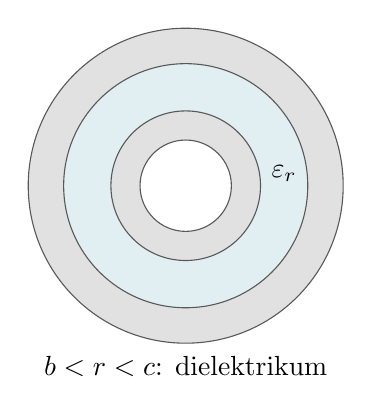
\begin{tikzpicture}[scale=1.0,>=Latex]
  \fill[ConductorGray,even odd rule] (0,0) circle (2.0) (0,0) circle (1.55);
  \fill[DielectricTint,even odd rule] (0,0) circle (1.55) (0,0) circle (0.95);
  \fill[ConductorGray,even odd rule] (0,0) circle (0.95) (0,0) circle (0.58);
  \foreach \r in {0.58,0.95,1.55,2.0}{\draw[black!65] (0,0) circle (\r);}
  \node at (1.25,0.15) {$\varepsilon_r$};
  \node at (0,-2.30) {$b<r<c$: dielektrikum};
\end{tikzpicture}
\end{minipage}\hfill
\begin{minipage}[c]{0.53\linewidth}
\[
 Q_{f,a}=0,\quad Q_{f,b}=Q_1,\quad Q_{f,c}=-Q_1,\quad Q_{f,d}=Q_1+Q_2.
\]
\[
 \sigma_{f,a}=0,\quad \sigma_{f,b}=\frac{Q_1}{4\pi b^2},\quad
 \sigma_{f,c}=-\frac{Q_1}{4\pi c^2},\quad
 \sigma_{f,d}=\frac{Q_1+Q_2}{4\pi d^2}.
\]
I $b<r<c$:
\[
 \mathbf D=\frac{Q_1}{4\pi r^2}\hat r,
 \qquad
 \mathbf E=\frac{Q_1}{4\pi\varepsilon_0\varepsilon_r r^2}\hat r,
\]
\[
 \mathbf P=\frac{\varepsilon_r-1}{\varepsilon_r}\frac{Q_1}{4\pi r^2}\hat r,
 \qquad \rho_b=0.
\]
\end{minipage}
\end{casebox}

\begin{casebox}{Bundet ladning på de to dielektriske grænser}
\[
 \boxed{\sigma_{b,b}=-\frac{\varepsilon_r-1}{\varepsilon_r}\frac{Q_1}{4\pi b^2}},
 \qquad
 \boxed{\sigma_{b,c}=+\frac{\varepsilon_r-1}{\varepsilon_r}\frac{Q_1}{4\pi c^2}}.
\]
\begin{center}
\textbf{fri ladning = lagt på lederne}\qquad$\big|$\qquad\textbf{bundet ladning = materialets respons}
\end{center}
\end{casebox}

\begin{casebox}{Kapacitans: felt $\to$ potentialforskel $\to$ $C$}
\[
 \boxed{C=\frac{Q}{\Delta V}},\qquad
 \boxed{E\to\Delta V=-\int\mathbf E\cdot d\mathbf l\to C}.
\]
Sfærisk kondensator, vakuum i $b<r<c$:
\[
 \boxed{C_{\rm vakuum}=4\pi\varepsilon_0\frac{bc}{c-b}}.
\]
Hele feltområdet fyldt med homogent lineært dielektrikum:
\[
 \boxed{C_{\rm diel}=4\pi\varepsilon_0\varepsilon_r\frac{bc}{c-b}=\varepsilon_rC_{\rm vakuum}}.
\]
\textbf{Gamle opgaver:} nov21.2, feb22.2, feb23.2, nov23.4, feb24.2, nov25.3.
\end{casebox}

\newpage
\setcounter{section}{4}

\section*{DEL II - MAGNETFELT / VEKTORPOTENTIALE}
\phantomsection
\addcontentsline{toc}{section}{DEL II - MAGNETFELT / VEKTORPOTENTIALE}
\begin{center}
{\Large\bfseries B/A - visuelt problemløsningsatlas}\\[1mm]
{\small Først værktøjerne $\to$ derefter geometri/opgavetype. Samme struktur som E/V-delen.}
\end{center}
\begin{quickbox}{Sådan navigerer du B/A-delen}
\[
\boxed{\text{hvad er givet?}}\to
\boxed{\text{genkend geometrien}}\to
\boxed{\text{vælg metode}}
\]
\[
\boxed{\text{Ampère / Biot--Savart / }\mathbf A}
\to
\boxed{\mathbf B\text{ eller }\mathbf A}
\to
\boxed{\text{regn videre}}
\]
\begin{center}
\begin{tabular}{llll}
\textbf{BA0 Værktøjer} & \textbf{BA1 Felt-tests} & \textbf{BA2 Find $B/A$} & \textbf{BA3 Regioner}\\
\textbf{BA4 Kraft/bevægelse} & \textbf{BA5 Dipol} & \textbf{BA6 Vektorpotentiale} & \textbf{BA7 Materialer}
\end{tabular}
\end{center}
\end{quickbox}

\section*{BA0 - Grundligninger og centrale relationer}
\phantomsection
\addcontentsline{toc}{section}{BA0 - Grundligninger og centrale relationer}
\begin{multicols}{2}
\begin{quickbox}{Lorentzkraft}
\[
\boxed{\mathbf F_B=q\mathbf v\times\mathbf B},
\qquad F_B=|q|vB\sin\theta.
\]
\end{quickbox}
\begin{quickbox}{Kraft på strømførende leder}
\[
\boxed{d\mathbf F=I\,d\boldsymbol\ell\times\mathbf B}
\]
\[
\boxed{\mathbf F=I\mathbf L\times\mathbf B}\quad
\text{(lige leder, homogent felt).}
\]
\end{quickbox}
\begin{quickbox}{Biot--Savart}
\[
\boxed{d\mathbf B=\frac{\mu_0}{4\pi}\frac{I\,d\boldsymbol\ell'\times\hat{\mathbf R}}{R^2}},
\qquad
\mathbf B=\int d\mathbf B.
\]
\end{quickbox}
\begin{quickbox}{Ampère og Gauss for magnetisme}
\[
\boxed{\oint\mathbf B\cdot d\boldsymbol\ell=\mu_0I_{\rm enc}},
\qquad
\boxed{\nabla\times\mathbf B=\mu_0\mathbf J}
\]
\[
\boxed{\nabla\cdot\mathbf B=0},
\qquad
\boxed{\oint\mathbf B\cdot d\mathbf a=0}.
\]
\end{quickbox}
\begin{quickbox}{Vektorpotentiale}
\[
\boxed{\mathbf B=\nabla\times\mathbf A},
\qquad
\boxed{\nabla^2\mathbf A=-\mu_0\mathbf J}
\]
\[
\boxed{\mathbf A(\mathbf r)=\frac{\mu_0}{4\pi}\iiint
\frac{\mathbf J(\mathbf r')}{|\mathbf r-\mathbf r'|}\,d\tau'}.
\]
\end{quickbox}
\begin{quickbox}{Magnetisk dipol}
\[
\boxed{\mathbf m=I\mathbf A},\qquad
\boxed{\boldsymbol\tau=\mathbf m\times\mathbf B},
\qquad
\boxed{U=-\mathbf m\cdot\mathbf B}.
\]
\end{quickbox}
\end{multicols}

\section*{BA1 - Maxwell-ligninger og felt-tests}
\phantomsection
\addcontentsline{toc}{section}{BA1 - Maxwell-ligninger og felt-tests}
\begin{casebox}{B-relaterede recognition-regler}
\[
\boxed{\nabla\cdot\mathbf B=0\Rightarrow\text{ingen magnetiske monopoler}}
\]
\[
\boxed{\nabla\times\mathbf B=\mu_0\mathbf J\quad\text{(magnetostatik)}}
\]
\[
\boxed{\mathbf J=\frac1{\mu_0}\nabla\times\mathbf B}.
\]
\casemethod{er $\mathbf B(x,y,z)$ givet, så brug curl til at finde strømmen. Skal et foreslået $\mathbf B$ testes, skal divergensen være nul.}
\end{casebox}
\begin{quickbox}{Når tidsafhængighed senere tillades}
\[
\nabla\times\mathbf B=
\mu_0\mathbf J+\mu_0\varepsilon_0\frac{\partial\mathbf E}{\partial t}.
\]
Altså kan både strøm og et tidsvarierende elektrisk felt skabe et cirkulerende magnetfelt.
\end{quickbox}

\section*{BA2 - Find $B$ eller $A$ ud fra geometri}
\phantomsection
\addcontentsline{toc}{section}{BA2 - Find B/A fra geometri}
\begin{quickbox}{Beslutningstræ}
\[
\begin{array}{rcl}
\text{høj symmetri} &\to& \text{Ampère}\\
\text{endelig leder/bue/løkke} &\to& \text{Biot--Savart}\\
\text{flere strømkilder} &\to& \text{superposition}\\
\mathbf A\text{ givet} &\to& \mathbf B=\nabla\times\mathbf A
\end{array}
\]
\end{quickbox}

\begin{casebox}{Lang lige leder}
\begin{minipage}[c]{0.42\linewidth}\centering
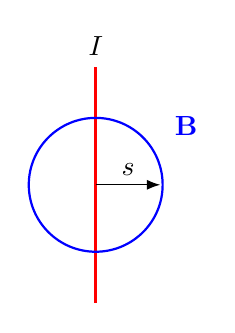
\begin{tikzpicture}[scale=1.0,>=Latex]
\draw[very thick,red] (0,-1.5)--(0,1.5) node[above,text=black] {$I$};
\draw[blue,thick,->] (0,0) circle (0.85);
\draw[->] (0,0)--(0.82,0) node[midway,above] {$s$};
\node[blue] at (1.15,0.75) {$\mathbf B$};
\end{tikzpicture}
\end{minipage}\hfill
\begin{minipage}[c]{0.54\linewidth}
\[
\boxed{\mathbf B(s)=\frac{\mu_0I}{2\pi s}\hat\phi}.
\]
\[
B(2\pi s)=\mu_0 I.
\]
\casemethod{højrehåndsregel giver den cirkulære retning.}
\end{minipage}
\end{casebox}

\begin{casebox}{Massiv strømførende cylinder, uniform $\mathbf J$}
\begin{center}
\begin{minipage}[t]{0.48\linewidth}\centering
\textbf{$s<R$}
\[
I_{\rm enc}=I\frac{s^2}{R^2},
\qquad
\boxed{B(s)=\frac{\mu_0Is}{2\pi R^2}}.
\]
\end{minipage}\hfill
\begin{minipage}[t]{0.48\linewidth}\centering
\textbf{$s>R$}
\[
I_{\rm enc}=I,
\qquad
\boxed{B(s)=\frac{\mu_0I}{2\pi s}}.
\]
\end{minipage}
\end{center}
\[
\boxed{I_{\rm enc}=\iint\mathbf J\cdot d\mathbf a}
\]
skal bruges først ved ikke-uniform $\mathbf J(s)$.
\end{casebox}

\begin{casebox}{Solenoide og toroide}
\begin{center}
\begin{minipage}[t]{0.48\linewidth}\centering
\textbf{Lang solenoide}
\[
\boxed{B_{\rm inde}\approx\mu_0nI},
\qquad
\boxed{B_{\rm ude}\approx0},
\qquad n=N/L.
\]
\end{minipage}\hfill
\begin{minipage}[t]{0.48\linewidth}\centering
\textbf{Ideal toroide}
\[
\boxed{B(s)=\frac{\mu_0NI}{2\pi s}}
\]
i viklingsområdet; idealiseret $B\approx0$ i centrum og udenfor.
\end{minipage}
\end{center}
\end{casebox}

\newpage
\section*{BA2 - Biot--Savart-geometrier \chaptertag{Kap. 5}}
\begin{casebox}{Endelig leder: generel Biot--Savart}
\[
\boxed{
\mathbf B(\mathbf r)=\frac{\mu_0I}{4\pi}\int
\frac{d\boldsymbol\ell'\times\hat{\mathbf R}}{R^2}},
\qquad
\mathbf R=\mathbf r-\mathbf r'.
\]
\casemethod{vælg $d\boldsymbol\ell'$ i strømretningen, skriv $\mathbf R$, brug symmetri og integrér.}
\end{casebox}
\begin{casebox}{Cirkulær bue og cirkulær løkke}
\begin{center}
\begin{minipage}[t]{0.48\linewidth}\centering
\textbf{Bue, centrum}
\[
\boxed{B_{\rm bue}=\frac{\mu_0I\phi}{4\pi R}}
\]
for buevinkel $\phi$ i radianer.
\end{minipage}\hfill
\begin{minipage}[t]{0.48\linewidth}\centering
\textbf{Løkke}
\[
\boxed{B(0)=\frac{\mu_0I}{2R}},
\qquad
\boxed{B(z)=\frac{\mu_0IR^2}{2(R^2+z^2)^{3/2}}}.
\]
\end{minipage}
\end{center}
\end{casebox}
\begin{casebox}{Flere ledere: superposition}
\[
\boxed{\mathbf B_{\rm total}=\sum_i\mathbf B_i}.
\]
Hvert bidrag beregnes med sin egen retning og lægges vektorielt sammen.
\end{casebox}
\textbf{Gamle opgaver:} nov24.3, jan25.5, dele af feb24.3.

\section*{BA3 - Region-for-region-problemer}
\phantomsection
\addcontentsline{toc}{section}{BA3 - Region-for-region}
\begin{quickbox}{Standardworkflow}
\[
\boxed{\text{opdel i regioner}\to I_{\rm enc}(s)\to\text{Ampère}\to B(s)}.
\]
Ved hver region: hvilken strøm omsluttes? kan Ampère bruges? hvilken retning har $B$? er der flere strømme?
\end{quickbox}
\begin{casebox}{Koaksiale strømme}
\[
s<a,\qquad a<s<b,\qquad b<s<c,\qquad s>c.
\]
I hver region:
\[
\boxed{B(s)=\frac{\mu_0I_{\rm enc}(s)}{2\pi s}}.
\]
\casepitfall{hold strømmenes fortegn/retning med i $I_{\rm enc}$; man trækker ikke felterne ved to grænser fra hinanden.}
\end{casebox}
\begin{casebox}{Hul/boring i strømleder: superposition}
\[
\boxed{\text{fysisk hul}=
\text{fuld strømfordeling }(+\mathbf J)+
\text{hjælpecylinder }(-\mathbf J)}
\]
\[
\boxed{\mathbf B_{\rm hul}=\mathbf B_{+\mathbf J}+\mathbf B_{-\mathbf J}}.
\]
Samme idé som hul i en ladningsfordeling i E/V-delen.
\end{casebox}
\textbf{Gamle opgaver:} juni21.3, feb22.4, feb24.4, nov25.4, nov21.5.

\newpage
\section*{BA4 - Kraft og bevægelse i kendt $\mathbf B$}
\phantomsection
\addcontentsline{toc}{section}{BA4 - Kraft og bevægelse i B}
\begin{casebox}{Ladet partikel: retning og størrelse}
\[
\boxed{\mathbf F_B=q\mathbf v\times\mathbf B},
\qquad
F_B=|q|vB\sin\theta.
\]
$q>0$: højrehåndsregel. $q<0$: vend retningen.
\[
v_\perp=v\sin\theta,\qquad v_\parallel=v\cos\theta.
\]
\casepitfall{magnetkraften står vinkelret på $\mathbf v$ og udfører ikke arbejde på en punktladning.}
\end{casebox}
\begin{casebox}{Cirkel, helix og acceleration gennem spænding}
\begin{center}
\begin{minipage}[t]{0.32\linewidth}\centering
\textbf{Cirkel}
\[
|q|vB=\frac{mv^2}{R},
\qquad
\boxed{R=\frac{mv}{|q|B}}.
\]
\end{minipage}
\begin{minipage}[t]{0.32\linewidth}\centering
\textbf{Helix}
\[
\boxed{R=\frac{mv_\perp}{|q|B}},
\qquad
v_\parallel=v\cos\theta.
\]
\end{minipage}
\begin{minipage}[t]{0.32\linewidth}\centering
\textbf{Efter spænding}
\[
|q|V=\frac12mv^2,
\quad
\boxed{R=\frac1B\sqrt{\frac{2mV}{|q|}}}.
\]
\end{minipage}
\end{center}
\end{casebox}
\begin{casebox}{Strømførende leder}
\[
\boxed{d\mathbf F=I\,d\boldsymbol\ell\times\mathbf B},
\qquad
\boxed{\mathbf F=I\mathbf L\times\mathbf B}.
\]
For krum leder i konstant $\mathbf B$:
\[
\boxed{\mathbf F=I(\mathbf r_{\rm slut}-\mathbf r_{\rm start})\times\mathbf B}.
\]
\casepitfall{$\int d\boldsymbol\ell$ er forskydningen, ikke buelængden.}
\end{casebox}
\begin{casebox}{To parallelle strømme}
\[
\boxed{\frac FL=\frac{\mu_0I_1I_2}{2\pi d}}.
\]
Samme retning $\Rightarrow$ tiltrækning; modsat retning $\Rightarrow$ frastødning.
\[
\boxed{I_1\to\mathbf B_1\to\mathbf F_2}.
\]
\end{casebox}
\textbf{Gamle opgaver:} juni21.3--4, feb22.3--4, feb24.3--4, nov25.4, jan25.5.

\section*{BA5 - Magnetisk dipol}
\phantomsection
\addcontentsline{toc}{section}{BA5 - Magnetisk dipol}
\begin{casebox}{Strømløkke som dipol}
\[
\boxed{\mathbf m=I\mathbf A},\qquad \mathbf A=A\hat n.
\]
For cirkulær løkke:
\[
\boxed{\mathbf m=I\pi R^2\hat n}.
\]
\casepitfall{$A$ er arealet omsluttet af strømvejen, ikke lederens tværsnitsareal og ikke vektorpotentialet.}
\end{casebox}
\begin{casebox}{Torque, energi og kraft}
\[
\boxed{\boldsymbol\tau=\mathbf m\times\mathbf B},
\qquad
\boxed{U=-\mathbf m\cdot\mathbf B}.
\]
I et inhomogent felt:
\[
\boxed{\mathbf F=\nabla(\mathbf m\cdot\mathbf B)}.
\]
\end{casebox}
\begin{casebox}{Roterende ladet ring}
\[
I=\frac{Q\omega}{2\pi},
\qquad
\boxed{m=\frac12Q\omega R^2}.
\]
\end{casebox}
\begin{casebox}{Dipolfelt og fjernfelt}
\[
\boxed{\mathbf B_{\rm dip}=
\frac{\mu_0}{4\pi r^3}
\left[3(\mathbf m\cdot\hat r)\hat r-\mathbf m\right]}.
\]
For $\mathbf m=m\hat z$:
\[
\boxed{\mathbf B_{\rm dip}=
\frac{\mu_0m}{4\pi r^3}
(2\cos\theta\,\hat r+\sin\theta\,\hat\theta)}.
\]
Ingen magnetisk monopol:
\[
\nabla\cdot\mathbf B=0,\qquad
\text{dipol}\to\text{quadrupol}\to\cdots.
\]
\end{casebox}
\textbf{Gamle opgaver:} feb22.7, feb23.4, jan26.4.

\section*{BA6 - Find $\mathbf A$ og brug $\mathbf A$ til at finde $\mathbf B$}
\phantomsection
\addcontentsline{toc}{section}{BA6 - Vektorpotentiale}
\begin{quickbox}{Recognition og workflow}
\[
\boxed{\mathbf J\to\mathbf A\to\mathbf B=\nabla\times\mathbf A}
\]
Hvis $\mathbf A$ er givet direkte:
\[
\boxed{\mathbf A\to\nabla\times\mathbf A\to\mathbf B}.
\]
\end{quickbox}
\begin{casebox}{Integralformer}
\[
\mathbf A(\mathbf r)=\frac{\mu_0I}{4\pi}\int\frac{d\boldsymbol\ell'}{|\mathbf r-\mathbf r'|}
\]
\[
\mathbf A(\mathbf r)=\frac{\mu_0}{4\pi}\iint
\frac{\mathbf K(\mathbf r')}{|\mathbf r-\mathbf r'|}\,da'
\]
\[
\boxed{\mathbf A(\mathbf r)=\frac{\mu_0}{4\pi}\iiint
\frac{\mathbf J(\mathbf r')}{|\mathbf r-\mathbf r'|}\,d\tau'}.
\]
\end{casebox}
\begin{casebox}{Poisson/Laplace for en fast kartesisk komponent}
\[
\boxed{\nabla^2\mathbf A=-\mu_0\mathbf J},
\qquad
\mathbf J=0\Rightarrow\nabla^2\mathbf A=0.
\]
Hvis $\mathbf A=A_z(s)\hat z$:
\[
\boxed{\frac1s\frac{d}{ds}\left(s\frac{dA_z}{ds}\right)=-\mu_0J_z(s)}.
\]
\casepitfall{for sfæriske komponenter $A_r,A_\theta,A_\phi$ må man generelt ikke ukritisk bruge den skalare Laplace-operator komponentvis.}
\end{casebox}
\begin{quickbox}{Parallel til E/V}
\[
\boxed{\rho\to V\to\mathbf E}
\qquad\leftrightarrow\qquad
\boxed{\mathbf J\to\mathbf A\to\mathbf B}.
\]
\end{quickbox}

\newpage
\section*{BA7 - Magnetiske materialer}
\phantomsection
\addcontentsline{toc}{section}{BA7 - Magnetiske materialer}
\begin{casebox}{Magnetisering og bundne strømme}
\[
\boxed{\mathbf M=\frac{d\mathbf m}{d\tau}},
\qquad
\boxed{\mathbf J_b=\nabla\times\mathbf M},
\qquad
\boxed{\mathbf K_b=\mathbf M\times\hat n}.
\]
\[
\boxed{\mathbf M\to\mathbf J_b,\mathbf K_b\to\mathbf B}.
\]
\end{casebox}
\begin{casebox}{$\mathbf H$: brug kun fri strøm}
\[
\boxed{\mathbf H=\frac1{\mu_0}\mathbf B-\mathbf M}
\quad\Longleftrightarrow\quad
\boxed{\mathbf B=\mu_0(\mathbf H+\mathbf M)}.
\]
\[
\boxed{\nabla\times\mathbf H=\mathbf J_f},
\qquad
\boxed{\oint\mathbf H\cdot d\boldsymbol\ell=I_{f,\rm enc}}.
\]
\[
\boxed{\mathbf H\text{ bruger fri strøm}}.
\]
\end{casebox}
\begin{casebox}{Lineært magnetisk medium}
\[
\mathbf M=\chi_m\mathbf H,
\qquad
\boxed{\mathbf B=\mu\mathbf H},
\]
\[
\mu=\mu_0(1+\chi_m),
\qquad
\mu_r=1+\chi_m.
\]
Standardworkflow:
\[
\boxed{I_{f,\rm enc}\to H\to B}.
\]
Samme geometrier som tidligere: solenoide, toroide og cylinder.
\end{casebox}
\begin{casebox}{Standard magnetiseret cylinder}
For
\[
\mathbf M=ks^2\hat z
\]
i en lang cylinder:
\[
\boxed{\mathbf J_b=-2ks\,\hat\phi},
\qquad
\boxed{\mathbf K_b=kR^2\hat\phi}\quad(s=R).
\]
\end{casebox}
\begin{quickbox}{Kapitel 4 $\leftrightarrow$ kapitel 6}
\[
\mathbf P\leftrightarrow\mathbf M,\qquad
\mathbf D\leftrightarrow\mathbf H,
\]
\[
\rho_b=-\nabla\cdot\mathbf P
\leftrightarrow
\mathbf J_b=\nabla\times\mathbf M,
\qquad
\sigma_b=\mathbf P\cdot\hat n
\leftrightarrow
\mathbf K_b=\mathbf M\times\hat n.
\]
\end{quickbox}
\textbf{Gamle opgaver:} nov22.5, nov24.6.

\newpage
\section*{DEL III - TIDSAFHÆNGIGE ELEKTROMAGNETISKE FELTER}
\phantomsection
\addcontentsline{toc}{section}{DEL III - TIDSAFHÆNGIGE ELEKTROMAGNETISKE FELTER}
\begin{center}
{\Large\bfseries DYN - visuelt problemløsningsatlas}\\[1mm]
{\small Grundligninger først $\to$ vælg dynamisk case $\to$ følg workflow.}
\end{center}
\begin{quickbox}{Den fysiske kobling}
\[
\boxed{\frac{\partial\mathbf B}{\partial t}\to\text{cirkulerende }\mathbf E}
\qquad
\boxed{\frac{\partial\mathbf E}{\partial t}\to\text{cirkulerende }\mathbf B}.
\]
\end{quickbox}

\newpage
\section*{DYN0 - Grundligninger og centrale relationer}
\phantomsection
\addcontentsline{toc}{section}{DYN0 - Grundligninger og centrale relationer}
\begin{multicols}{2}
\begin{quickbox}{Strøm og ledningsevne}
\[
\boxed{\mathbf J=\sigma_c\mathbf E},
\qquad
\boxed{I=\iint\mathbf J\cdot d\mathbf a}
\]
\[
\boxed{R=\frac VI},
\qquad
\boxed{R=\frac{L}{\sigma_cA}}\quad\text{(homogen leder).}
\]
\end{quickbox}
\begin{quickbox}{Magnetisk flux og Faraday}
\[
\boxed{\Phi_B=\iint\mathbf B\cdot d\mathbf a},
\qquad
\Phi_B=BA\cos\theta
\]
\[
\boxed{\mathcal E=-\frac{d\Phi_B}{dt}},
\qquad
\boxed{\mathcal E=-N\frac{d\Phi_B}{dt}}.
\]
\end{quickbox}
\begin{quickbox}{Motional EMF}
\[
\boxed{\mathcal E=\oint(\mathbf v\times\mathbf B)\cdot d\boldsymbol\ell}
\]
\[
\boxed{\mathcal E=BLv}\quad\text{(standardstang).}
\]
\end{quickbox}
\begin{quickbox}{Induceret elektrisk felt}
\[
\boxed{\oint\mathbf E\cdot d\boldsymbol\ell=-\frac{d\Phi_B}{dt}}
\]
\[
\boxed{\nabla\times\mathbf E=-\frac{\partial\mathbf B}{\partial t}}.
\]
\end{quickbox}
\begin{quickbox}{Induktion og energi}
\[
\boxed{N\Phi_B=LI},
\qquad
\boxed{\mathcal E_L=-L\frac{dI}{dt}}
\]
\[
\boxed{N_2\Phi_{21}=MI_1},
\qquad
\boxed{\mathcal E_2=-M\frac{dI_1}{dt}}
\]
\[
\boxed{U_B=\frac12LI^2}.
\]
\end{quickbox}
\begin{quickbox}{Ampère--Maxwell}
\[
\boxed{I_d=\varepsilon_0\frac{d\Phi_E}{dt}}
\]
\[
\boxed{\oint\mathbf B\cdot d\boldsymbol\ell=
\mu_0\left(I_{\rm enc}+\varepsilon_0\frac{d\Phi_E}{dt}\right)}.
\]
\end{quickbox}
\end{multicols}

\section*{DYN1 - Beslutningstræ: hvilken dynamisk metode?}
\phantomsection
\addcontentsline{toc}{section}{DYN1 - Vælg induktionsmetode}
\begin{casebox}{Recognition map}
\[
\begin{array}{rcl}
\text{leder bevæger sig i }B &\to& \text{motional EMF}\\
\text{areal/geometri ændrer sig} &\to& \text{flux + Faraday}\\
B=B(t),\text{ fast løkke} &\to& \text{Faraday}\\
B(t)\to E &\to& \text{induceret elektrisk felt}\\
\text{egen strøm ændres} &\to& \text{selvinduktion}\\
I_1(t)\text{ påvirker kreds 2} &\to& \text{gensidig induktion}\\
E(t)\to B &\to& \text{Ampère--Maxwell}
\end{array}
\]
\end{casebox}

\section*{DYN2 - Strøm, ledningsevne og modstand}
\phantomsection
\addcontentsline{toc}{section}{DYN2 - Strøm og modstand}
\begin{casebox}{Homogen leder}
\[
\boxed{\mathbf J=\sigma_c\mathbf E},
\qquad
\boxed{I=JA},
\qquad
\boxed{R=\frac{L}{\sigma_cA}}.
\]
\end{casebox}
\begin{casebox}{Ikke-uniform ledningsevne}
\[
\boxed{\sigma_c(x)\to E(x)=\frac{J}{\sigma_c(x)}
\to \Delta V=-\int E\,dx\to J\to I\to R}.
\]
Når relevant:
\[
\boxed{\rho=\varepsilon_0\nabla\cdot\mathbf E}.
\]
\end{casebox}

\newpage
\section*{DYN3 - Bevægelig leder i homogent $\mathbf B$}
\phantomsection
\addcontentsline{toc}{section}{DYN3 - Bevægelig leder}
\begin{casebox}{Standardstang på skinner}
\[
\boxed{\mathcal E=BLv}
\to
\boxed{I=\frac{BLv}{R}}
\to
\boxed{F=ILB}.
\]
\[
\boxed{P_{\rm mek}=Fv},
\qquad
\boxed{P_R=I^2R},
\qquad
\boxed{W=\int P\,dt}.
\]
I den idealiserede konstante-hastighedscase uden anden energiændring:
\[
\boxed{P_{\rm mek}=P_R}.
\]
\end{casebox}
\textbf{Reference:} juni21.6.

\section*{DYN4 - Motional EMF med mekanisk feedback}
\phantomsection
\addcontentsline{toc}{section}{DYN4 - Mekanisk feedback}
\begin{casebox}{Batteri + bevægelig stang}
\[
\boxed{I(v)=\frac{V-Bdv}{R}}
\]
\[
I(v)\to F=IBd\to m\frac{dv}{dt}=F.
\]
Terminalhastighed:
\[
V-Bdv_\infty=0
\quad\Rightarrow\quad
\boxed{v_\infty=\frac{V}{Bd}}.
\]
Når differentialligningen har standardformen:
\[
\boxed{v(t)=v_\infty(1-e^{-t/\tau})}.
\]
Energiflow:
\[
\boxed{U_{\rm batt}\to K+Q_{\rm Joule}}.
\]
\end{casebox}
\textbf{Reference:} nov25.5.

\newpage
\section*{DYN5 - Ændrende geometri / areal}
\phantomsection
\addcontentsline{toc}{section}{DYN5 - Ændrende geometri}
\begin{casebox}{Arealet ændrer sig}
\[
\boxed{\text{geometri}\to A(t)\to\Phi_B(t)\to\mathcal E(t)\to I(t)\to F,P,W}.
\]
\[
\boxed{\text{geometrien ændrer sig}\Rightarrow\text{tænk flux først}}.
\]
For uniformt felt:
\[
\Phi_B(t)=B\,A(t)\cos\theta.
\]
\end{casebox}
\textbf{Reference:} feb24.5.

\section*{DYN6 - Fast geometri + $B(t)$}
\phantomsection
\addcontentsline{toc}{section}{DYN6 - B(t) i fast spole}
\begin{casebox}{Fast spole i tidsvarierende felt}
Hvis $A$ og vinklen er konstante:
\[
\boxed{\mathcal E=-NA\frac{dB}{dt}}.
\]
Derefter:
\[
\boxed{\mathcal E\to I(t)=\frac{\mathcal E}{R}\to P(t)=I^2R\to W=\int Pdt}.
\]
\end{casebox}
\begin{quickbox}{Lenz' lov}
\[
\boxed{\text{induktionen modvirker ændringen i flux}}
\neq
\boxed{\text{altid modsat det oprindelige }B}.
\]
Procedure: fluxretning $\to$ vokser/falder? $\to$ induceret $B$ $\to$ højrehåndsregel $\to I$.
\end{quickbox}

\section*{DYN7 - Induceret elektrisk felt}
\phantomsection
\addcontentsline{toc}{section}{DYN7 - Induceret E}
\begin{casebox}{Tidsvarierende $B$ skaber cirkulerende $E$}
\[
\boxed{\oint\mathbf E\cdot d\boldsymbol\ell=-\frac{d\Phi_B}{dt}}.
\]
Ved cirkelsymmetri:
\[
\boxed{E(2\pi s)=-\frac{d\Phi_B}{dt}}.
\]
Der behøver ikke være en fysisk ledning.
\end{casebox}
\begin{casebox}{Begrænset cylindrisk $B(t)$-område}
Hvis $B(t)$ kun findes for $s<R$:
\[
s<R:\quad \Phi_B=\pi s^2B(t),
\]
\[
s>R:\quad \Phi_B=\pi R^2B(t).
\]
Brug derefter Faradays integralform separat i de to regioner.
\end{casebox}

\newpage
\section*{DYN8 - Selvinduktion}
\phantomsection
\addcontentsline{toc}{section}{DYN8 - Selvinduktion}
\begin{casebox}{Samme kreds laver feltet og oplever fluxen}
\[
\boxed{I\to B\to\Phi_B\to L}
\]
\[
\boxed{L=\frac{N\Phi_B}{I}},
\qquad
\boxed{\mathcal E_L=-L\frac{dI}{dt}}.
\]
\[
\boxed{\text{selvinduktion modvirker ændringen i }I}.
\]
\end{casebox}

\section*{DYN9 - Gensidig induktion}
\phantomsection
\addcontentsline{toc}{section}{DYN9 - Gensidig induktion}
\begin{casebox}{To separate kredse}
\[
\boxed{I_1\to B_1\to\Phi_{21}\to M}
\]
\[
\boxed{M=\frac{N_2\Phi_{21}}{I_1}},
\qquad
\boxed{\mathcal E_2=-M\frac{dI_1}{dt}}.
\]
For passive lineære kredse:
\[
M_{12}=M_{21}.
\]
\end{casebox}

\section*{DYN10 - Magnetisk energi}
\phantomsection
\addcontentsline{toc}{section}{DYN10 - Magnetisk energi}
\begin{casebox}{Energi lagret i induktans/felt}
\[
\boxed{U_B=\frac12LI^2}.
\]
Effekt:
\[
\boxed{P=\mathcal E I}.
\]
I vakuum:
\[
\boxed{U_B=\frac1{2\mu_0}\iiint B^2\,d\tau}.
\]
\end{casebox}

\newpage
\section*{DYN11 - Forskydningsstrøm og Ampère--Maxwell}
\phantomsection
\addcontentsline{toc}{section}{DYN11 - Ampere-Maxwell}
\begin{casebox}{Opladende kondensator}
\[
\boxed{I_d=\varepsilon_0\frac{d\Phi_E}{dt}}
\]
\[
\boxed{\oint\mathbf B\cdot d\boldsymbol\ell=
\mu_0(I_{\rm enc}+I_d)}.
\]
For ideal kondensator:
\[
\boxed{I_d=I}.
\]
\casemethod{vælg Ampère-løkke; mellem pladerne erstatter den tidsvarierende elektriske flux den manglende ledningsstrøm gennem fladen.}
\end{casebox}

\section*{DYN12 - Maxwell samlet}
\phantomsection
\addcontentsline{toc}{section}{DYN12 - Maxwell samlet}
\begin{casebox}{De fire Maxwell-ligninger}
\[
\boxed{\nabla\cdot\mathbf E=\frac{\rho}{\varepsilon_0}},
\qquad
\boxed{\nabla\cdot\mathbf B=0}
\]
\[
\boxed{\nabla\times\mathbf E=-\frac{\partial\mathbf B}{\partial t}},
\qquad
\boxed{\nabla\times\mathbf B=
\mu_0\mathbf J+\mu_0\varepsilon_0\frac{\partial\mathbf E}{\partial t}}.
\]
\end{casebox}
\begin{quickbox}{Samlet fysisk kort}
\[
\boxed{\rho\to\mathbf E}
\qquad
\boxed{\mathbf J\to\mathbf B}
\]
\[
\boxed{\frac{\partial\mathbf B}{\partial t}\to\text{cirkulerende }\mathbf E}
\qquad
\boxed{\frac{\partial\mathbf E}{\partial t}\to\text{cirkulerende }\mathbf B}.
\]
\[
\boxed{B(t)\to E\quad\text{Faraday}}
\qquad
\boxed{E(t)\to B\quad\text{Ampère--Maxwell}}.
\]
\end{quickbox}

\begin{quickbox}{Hvad kan man regne videre til?}
Typiske kæder:
\[
\boxed{B\to\mathcal E\to I\to F\to P\to W}
\]
\[
\boxed{I\to B\to\Phi_B\to L\to U_B}.
\]
\end{quickbox}

\textbf{Gamle opgaver:} juni21.6, feb22.6, nov22.3, nov22.6, feb23.5, nov23.2, nov23.5, feb24.5, nov24.4, nov24.5, jan25.6, nov25.5, jan26.3.


\section{Eksamen - beslutningstræ}
\begin{quickbox}{Hvilken metode skal jeg prøve først?}
\begin{tabularx}{\textwidth}{>{\bfseries}p{4.0cm}X}
Punktladninger & Coulomb + superposition.\\
Kontinuert ladning uden høj symmetri & $dq$ + Coulomb/potentialintegral.\\
Kugle/cylinder/plan med høj symmetri & Gauss.\\
Flere radiale grænser & Vælg region + generel Gauss-radius; find $Q_{\rm enc}$ direkte.\\
Givet $\mathbf E$ eller $V$ & grad/div/curl; $\mathbf E=-\nabla V$, $\rho=\epsz\nabla\cdot\mathbf E$.\\
Leder/hulrum & $E=0$ i lederen + Gauss + total ladning.\\
Strømleder, kompliceret geometri & Biot-Savart.\\
Lang symmetrisk strømgeometri & Ampère.\\
Givet $\mathbf A$ & $\mathbf B=\nabla\times\mathbf A$.\\
Bevægende leder & motional EMF.\\
Ændrende magnetisk flux & Faraday + Lenz.\\
Ændrende elektrisk flux & Ampère-Maxwell.\\
\end{tabularx}
\end{quickbox}

\vfill
\small\textit{Masterprincip: denne fil opdateres løbende, når gamle eksamensopgaver afslører nye standardmetoder, faldgruber eller nyttige standardresultater.}
\end{document}
